
\section{Pre-fit data-MC}
\label{sec:strong:dataMC}
In this section we show the pre-fit agreement between data and the \gls{mc} simulation before the fit in the \gls{cr}
in the distribution of the same kinematic variables as in Section \ref{sec:strong:sigbkg}. 
All the plots show in this section do not include systematic uncertainties and include all the relevant \gls{mc} \glspl{sf}. 
In order to investigate a region of the phase space depleted in signal events the requirement on the number
of b-tagged jets is relaxed to $\nbjet \geq 2$. 

\subsection{Kinematic reweighting}
\label{sec:strong:kinrw}

The modelling of most kinematic variables related to the energy of the event shows a moderate disagreement 
when compared with data in the 1-lepton channel, while in the agreement is good in the 0-lepton channel. 
This is particularly visible in the distribution of \meff, as shown in Figure \ref{fig:strong:datamc:meff_prerw}.

\begin{figure*}[h]
\centering 
\subfigure[]{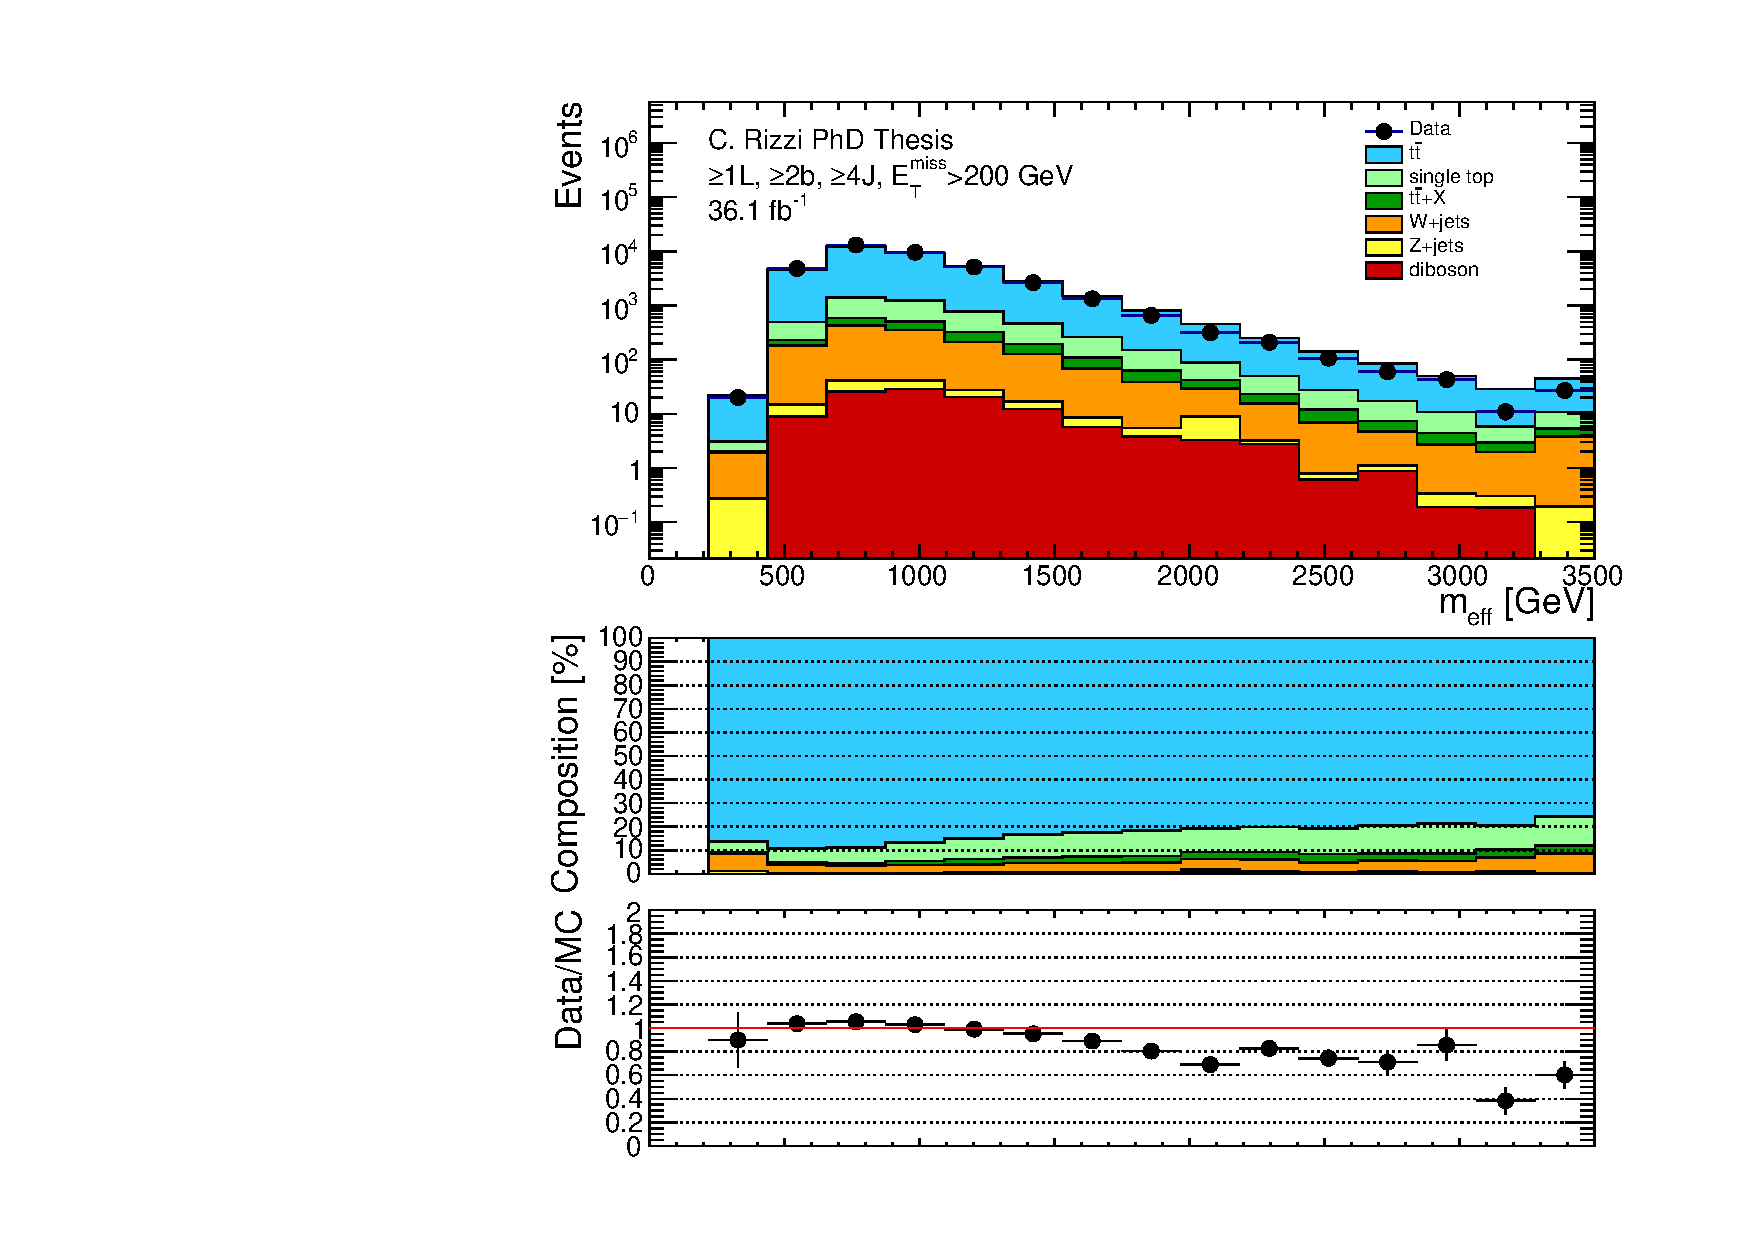
\includegraphics[width=0.49\textwidth]{figures/strong_prod/data_mc/1L_2bin/data_mc_meff_incl.pdf}
\label{fig:strong:datamc:meff_prerw_1L}}
\subfigure[]{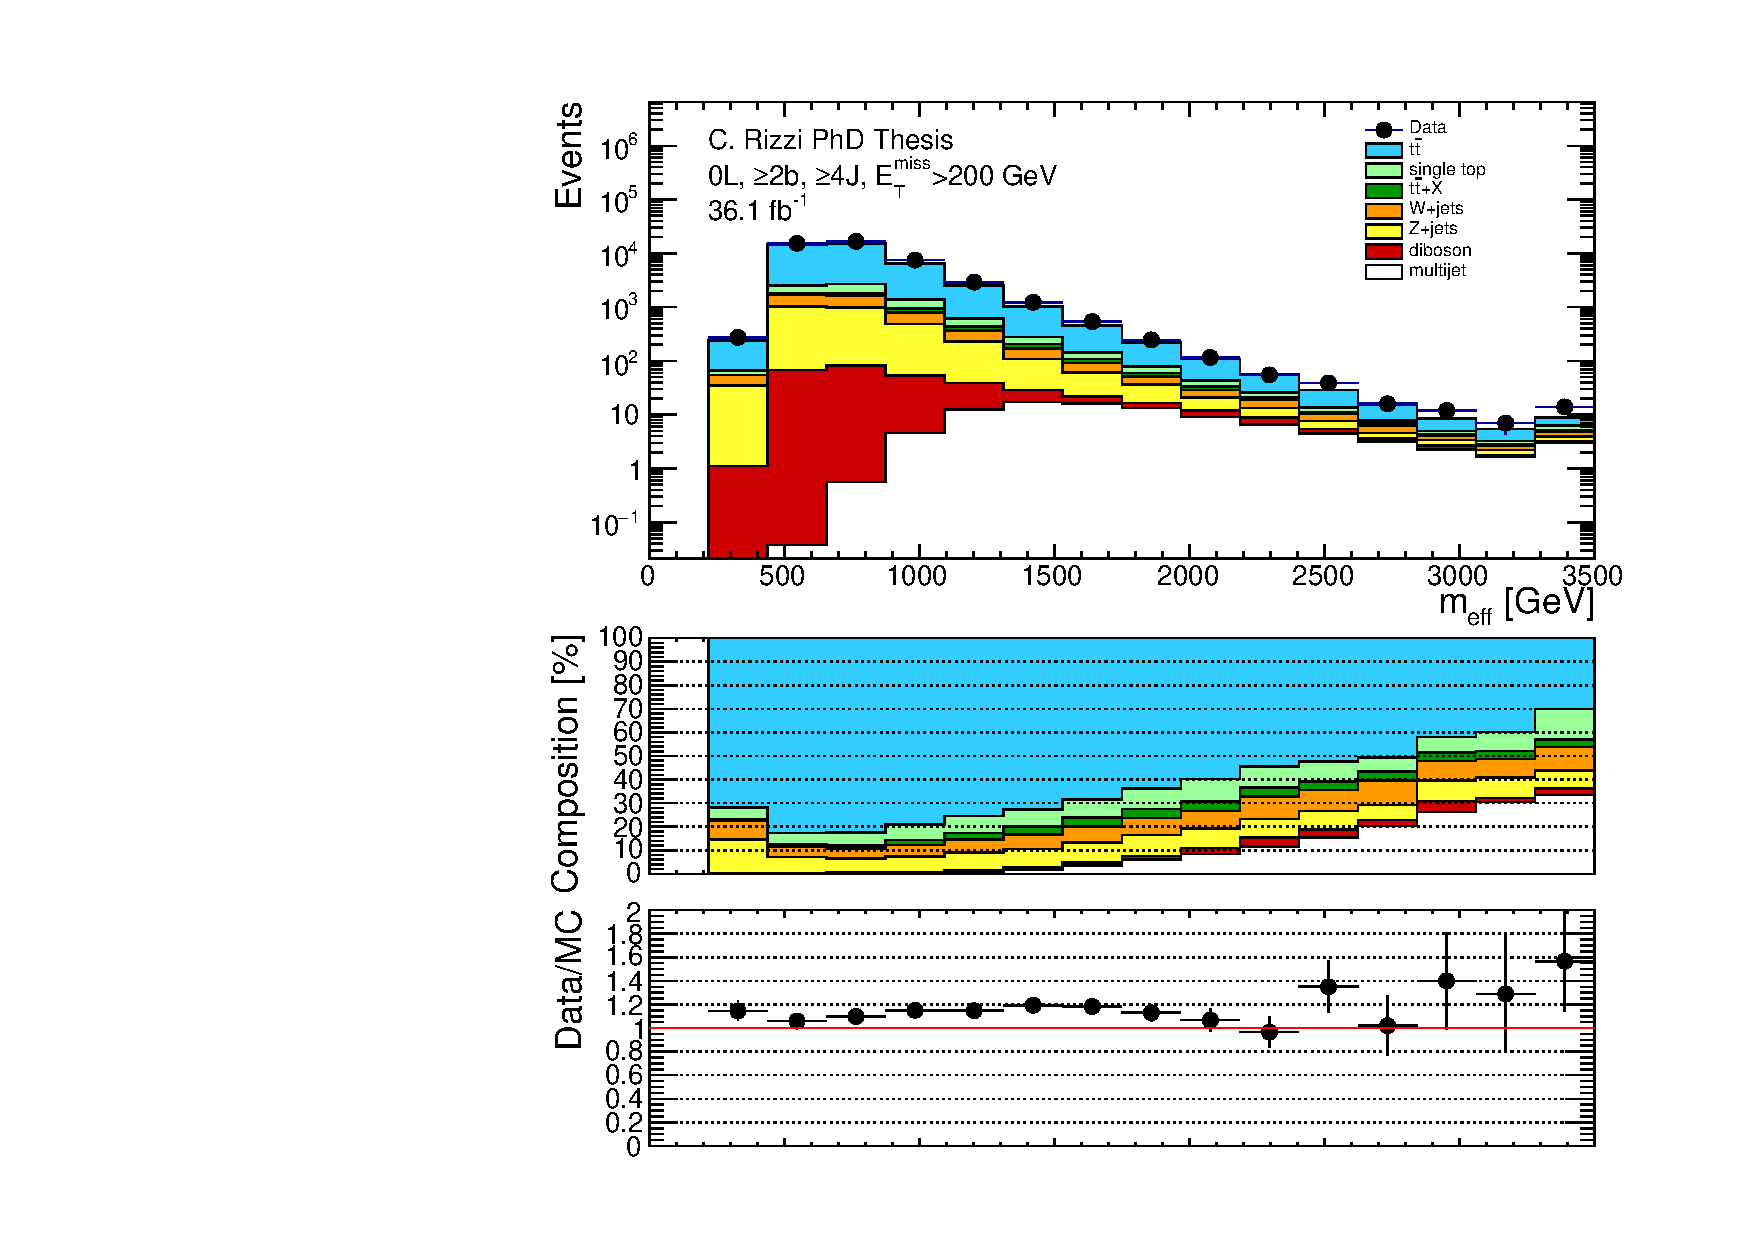
\includegraphics[width=0.49\textwidth]{figures/strong_prod/data_mc/0L_2bin/data_mc_meff_incl.pdf}
\label{fig:strong:datamc:meff_prerw_0L}}
\caption{ \subref{fig:strong:datamc:meff_prerw_1L}
}
\label{fig:strong:datamc:meff_prerw}
\end{figure*}

While the downward trend in the data/MC ratio in the 1-lepton channel is clearly visible in the bottom panel of Figure \ref{fig:strong:datamc:meff_prerw_1L},
Figure \ref{fig:strong:datamc:meff_prerw_0L} shows that this is not present in the 0-lepton channel.
This difference in trends is problematic for the analysis, since all of the \glspl{vr} require at least one signal lepton, 
including the ones used to derive the prediction for 0-lepton \glspl{sr}. 

To mitigate this problem and to have a better estimate of the background in the high-\meff tail, a reweighting is derived 
based on the distribution of \meff in a region that requires exactly two b-jets and low \mtb and is therefore
 orthogonal to all the analysis regions. More details on the reweighting procedure and on its validation are given in Appendix \ref{app:meffrw}.
All the plots in the rest of this section assume that the reweighting has already been applied. 


\subsection{Data-MC comparison after the reweighting}

Figures \ref{fig:strong:datamc1L_a} and \ref{fig:strong:datamc1L_b} show the data-MC agreement in the 1-lepton preselection after the 
kinematic reweighting described in the previous paragraph, while 
the agreement in the 0-lepton preselection is shown in Figures \ref{fig:strong:datamc0L_a} and \ref{fig:strong:datamc0L_b}.
The 1-lepton and 0-lepton preselection require:
\begin{itemize}
\item $\geq$ 4 jets,
\item $\geq$ 2 b-jets,
\item $\met > 200$ GeV
\end{itemize}
and respectively at least one signal lepton or a lepton veto and $\dphimin > 0.4$.

In Figure \ref{fig:strong:datamc1L:meff_incl} it can be noted how the kinematic reweighting improves the data-MC agreement in
the 1-lepton channel. 
All the distributions shown appear well modelled, with the exception of the number of b-jets 
that shows an underestimate of \gls{mc} with respect to the data that increases with the number of b-jets, both in 
the 1-lepton channel and in the 0-lepton channel 
(Figures \ref{fig:strong:datamc1L:bjets_n} and \ref{fig:strong:datamc0L:bjets_n} respectively).
This mismodelling does not constitute a problem in this analysis, 
since the \glspl{cr} have the same b-jet multiplicity as the corresponding \glspl{sr}.



\begin{figure*}[htbp]
\centering 
\subfigure[\meff]{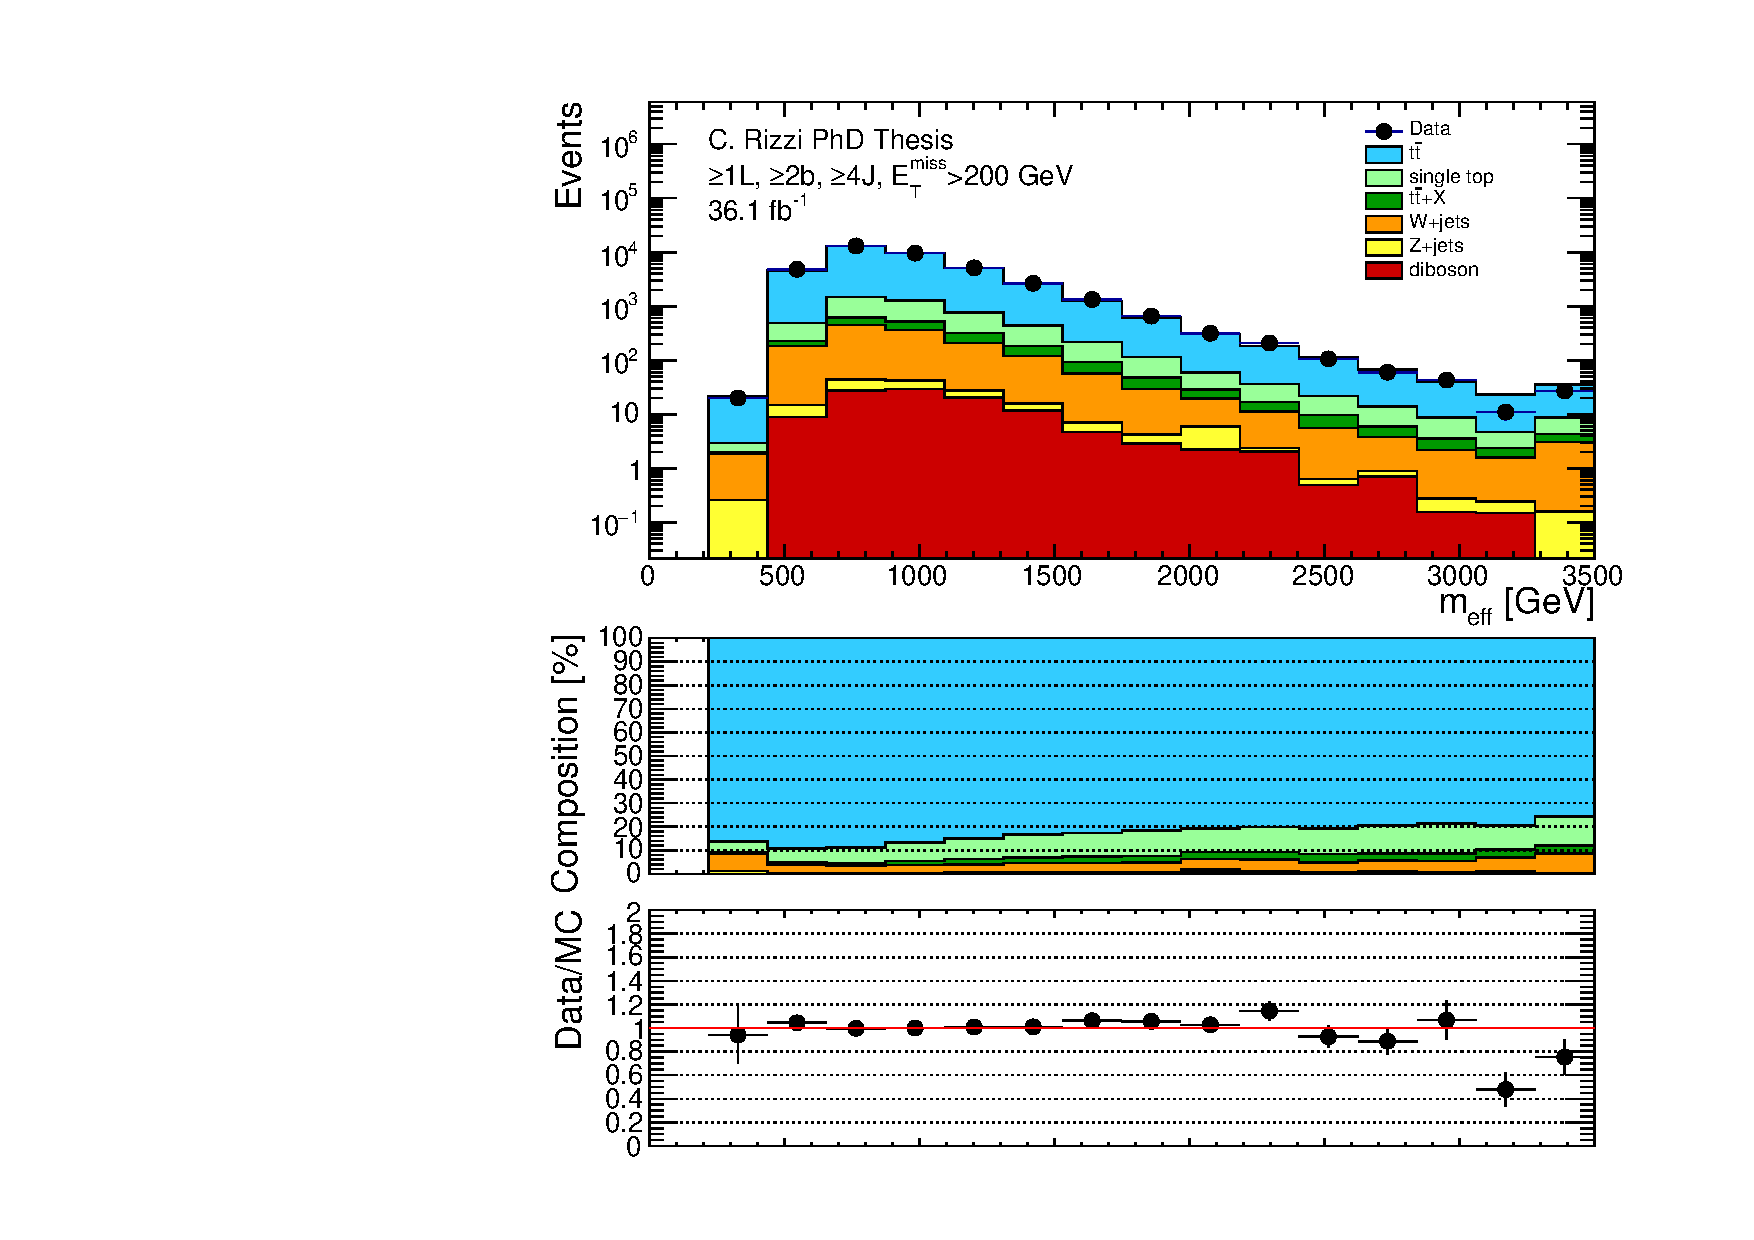
\includegraphics[width=0.45\textwidth]{figures/strong_prod/data_mc/1L_2bin_rw/data_mc_meff_incl.pdf}
\label{fig:strong:datamc1L:meff_incl}}
\subfigure[\mjsum]{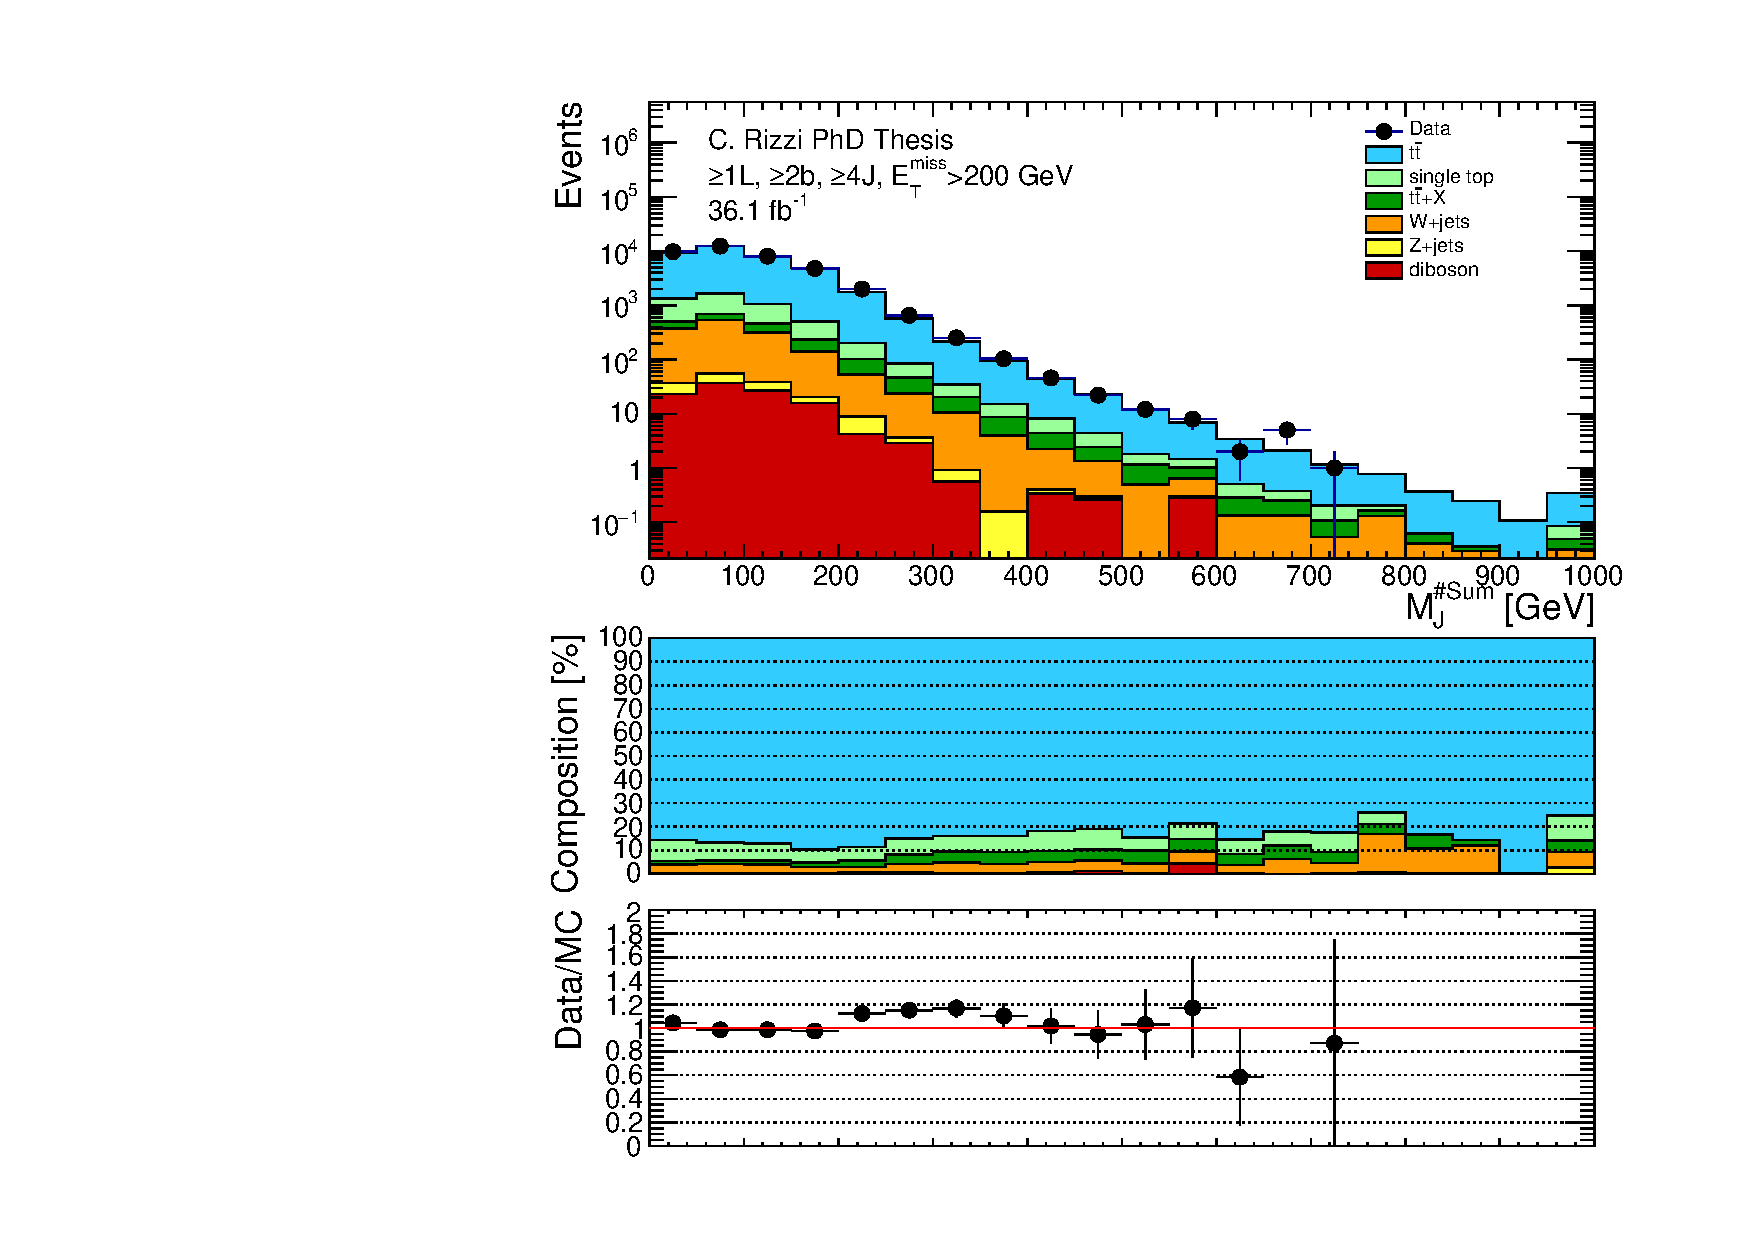
\includegraphics[width=0.45\textwidth]{figures/strong_prod/data_mc/1L_2bin_rw/data_mc_MJSum_rc_r08pt10.pdf}
\label{fig:strong:datamc1L:MJSum_rc_r08pt10}}\\
\subfigure[\met]{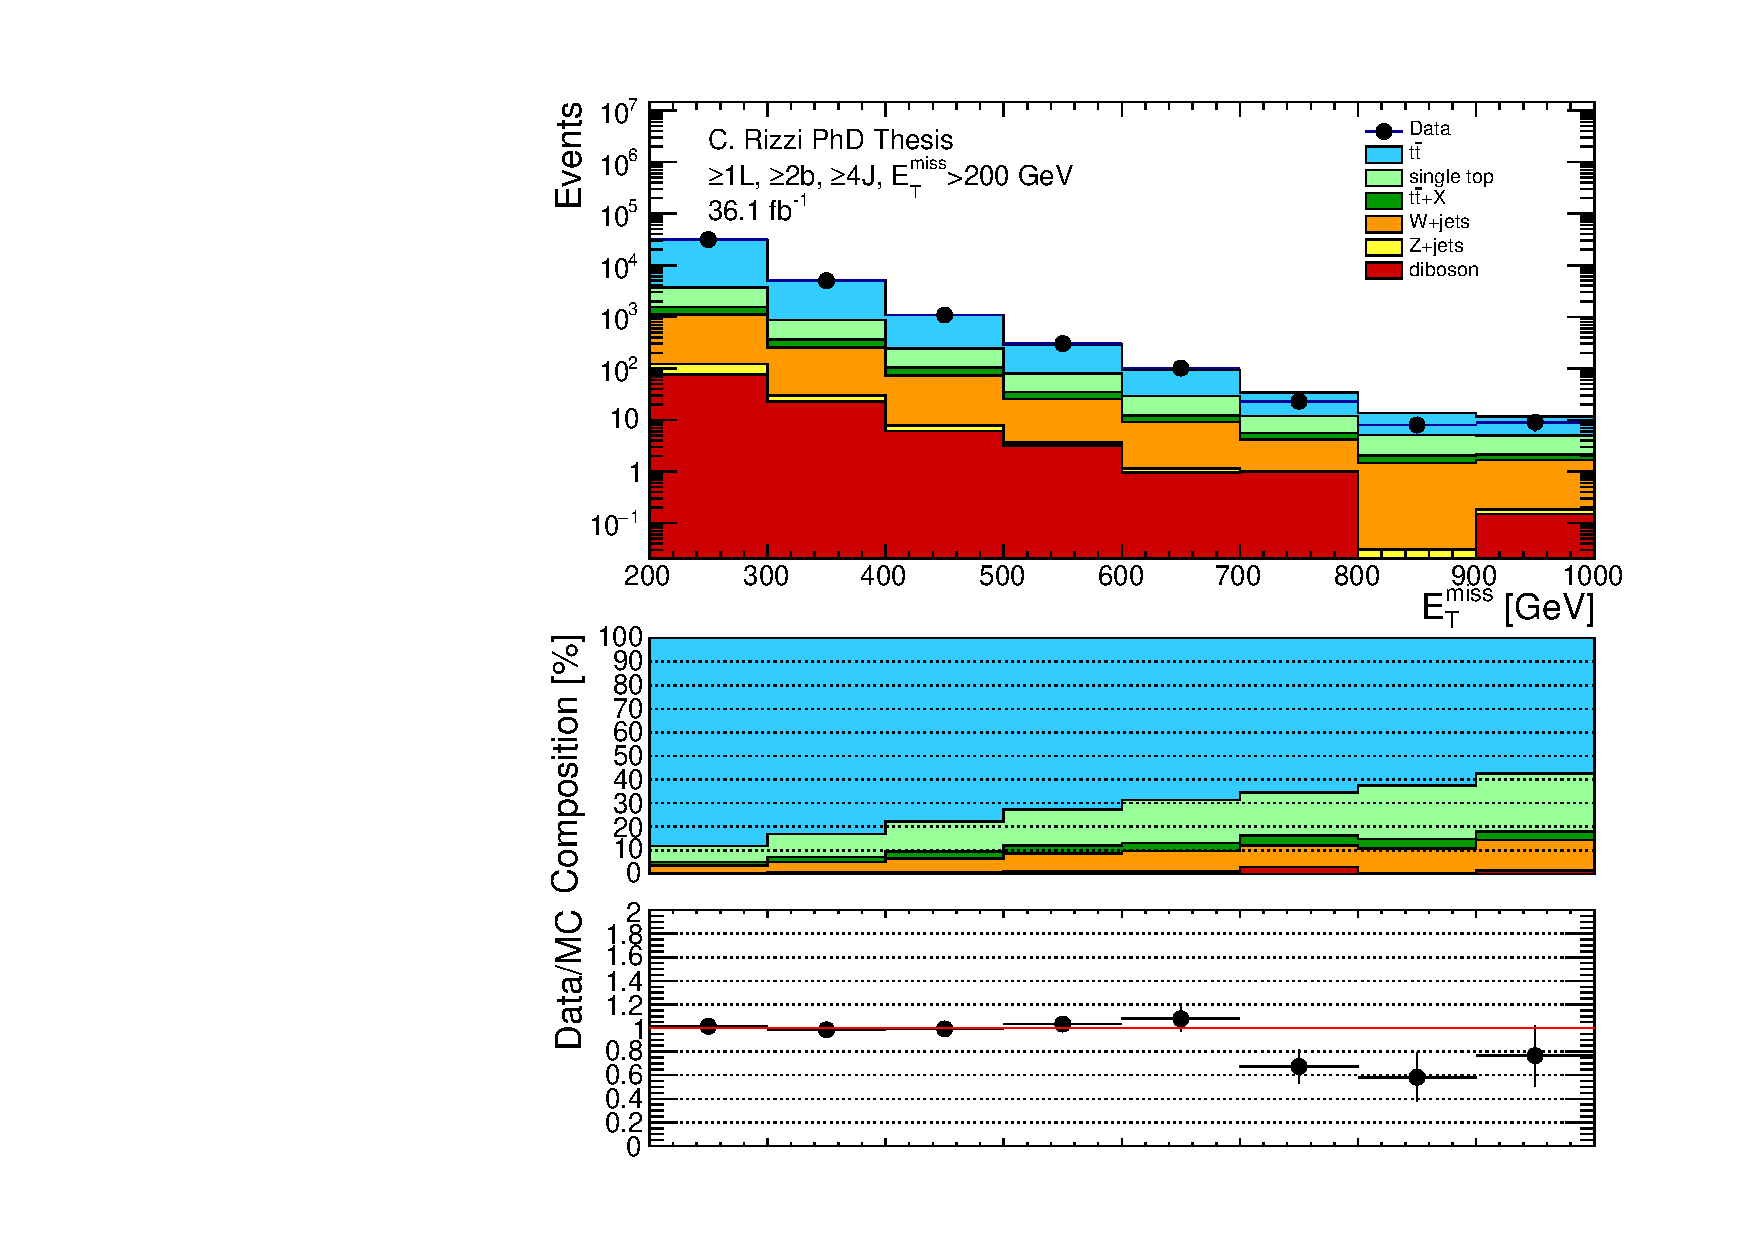
\includegraphics[width=0.45\textwidth]{figures/strong_prod/data_mc/1L_2bin_rw/data_mc_met.pdf}
\label{fig:strong:datamc1L:met}}
\subfigure[$\phi$(\met)]{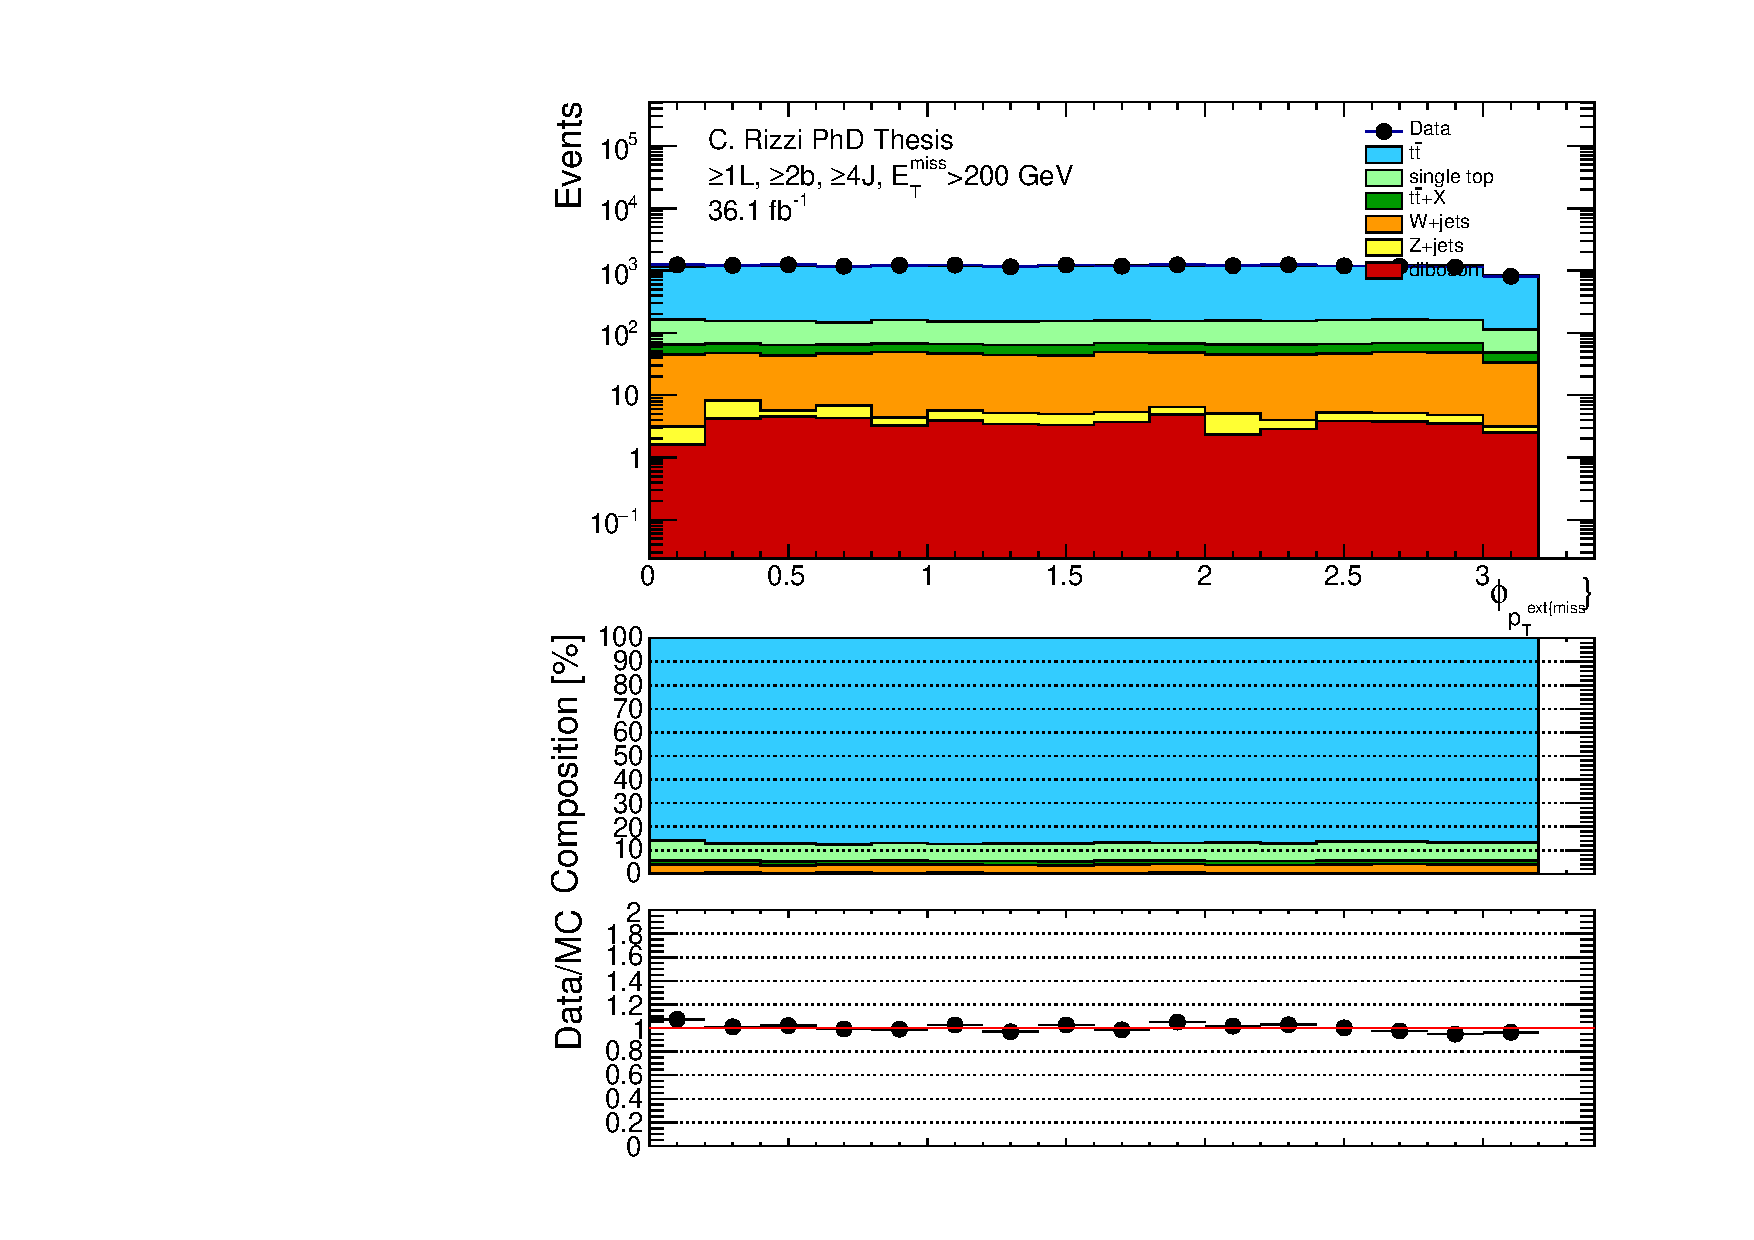
\includegraphics[width=0.45\textwidth]{figures/strong_prod/data_mc/1L_2bin_rw/data_mc_met_phi.pdf}
\label{fig:strong:datamc1L:met_phi}}\\
\subfigure[\mt]{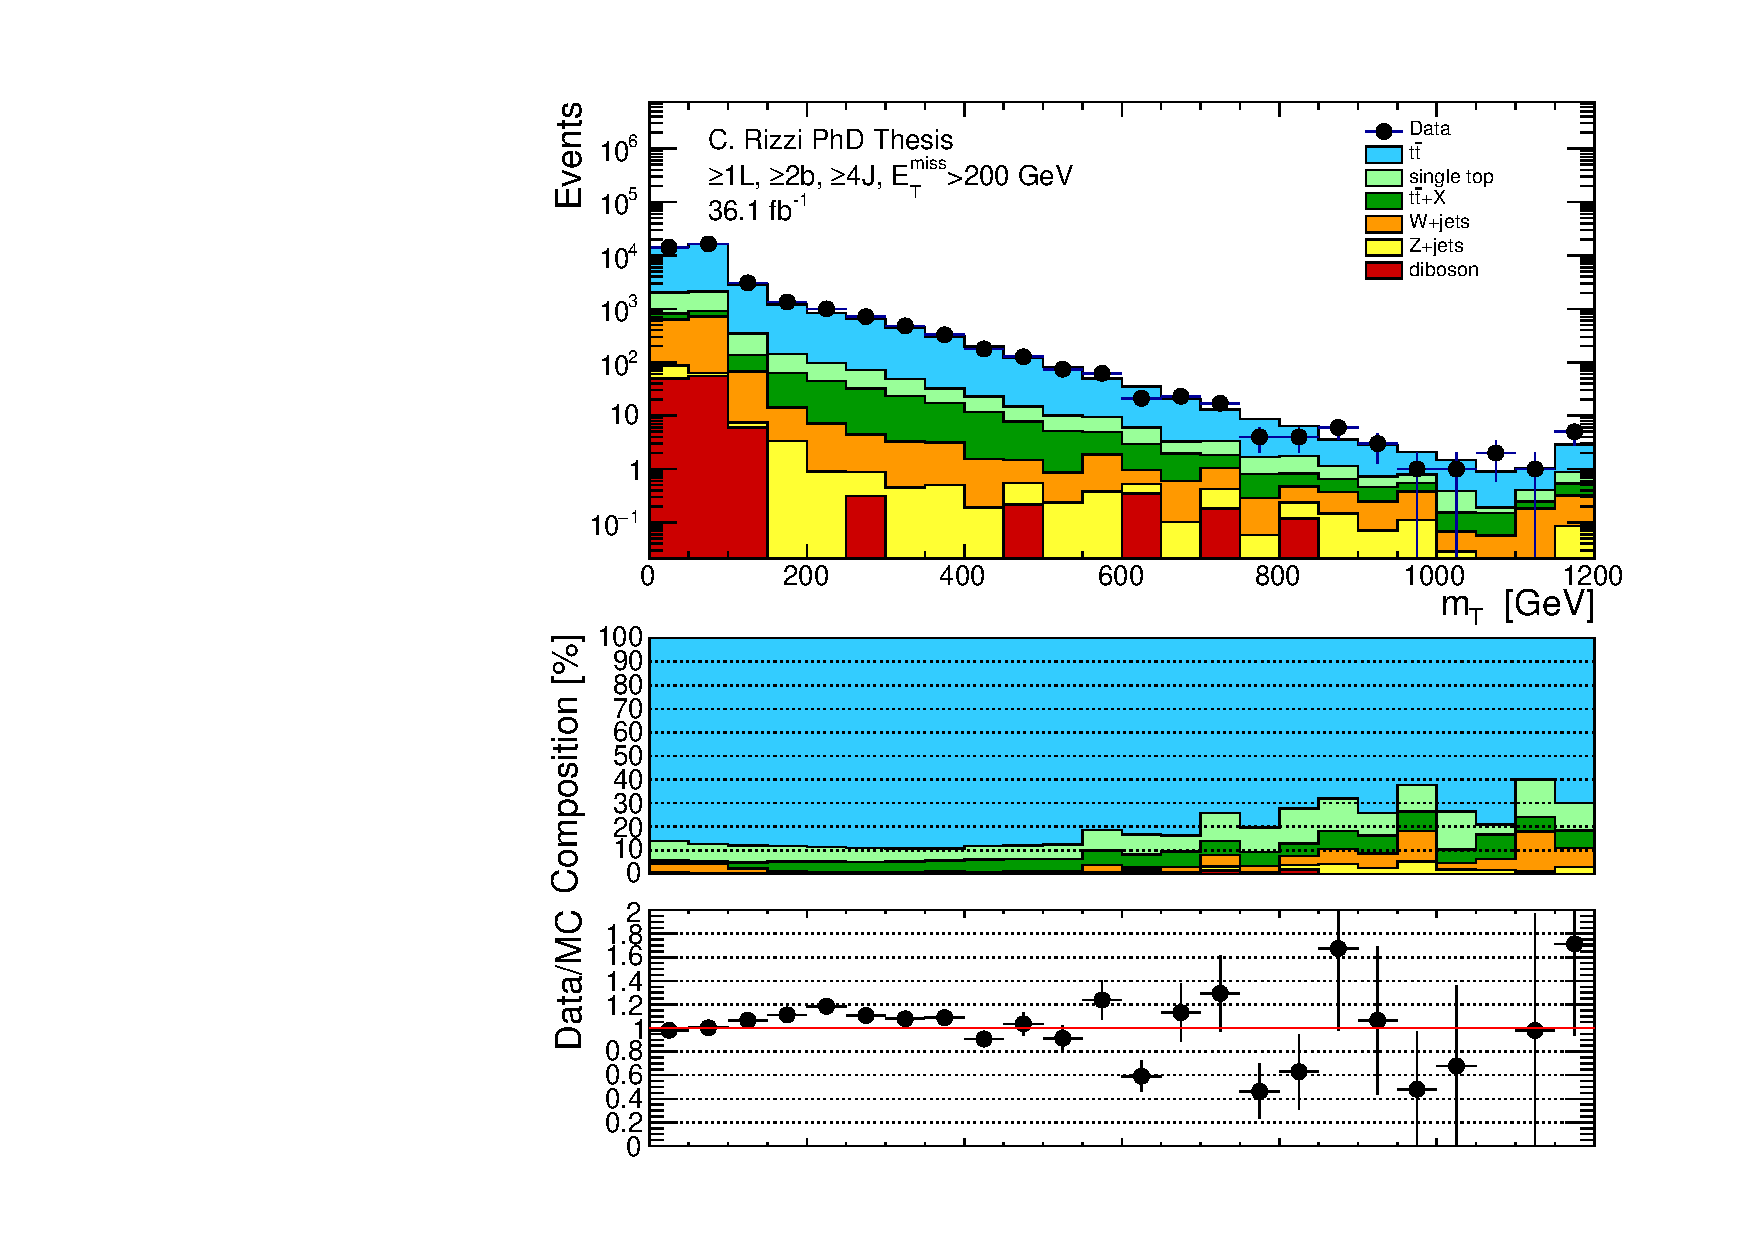
\includegraphics[width=0.45\textwidth]{figures/strong_prod/data_mc/1L_2bin_rw/data_mc_mT.pdf}
\label{fig:strong:datamc1L:mT}}
\subfigure[\mtb]{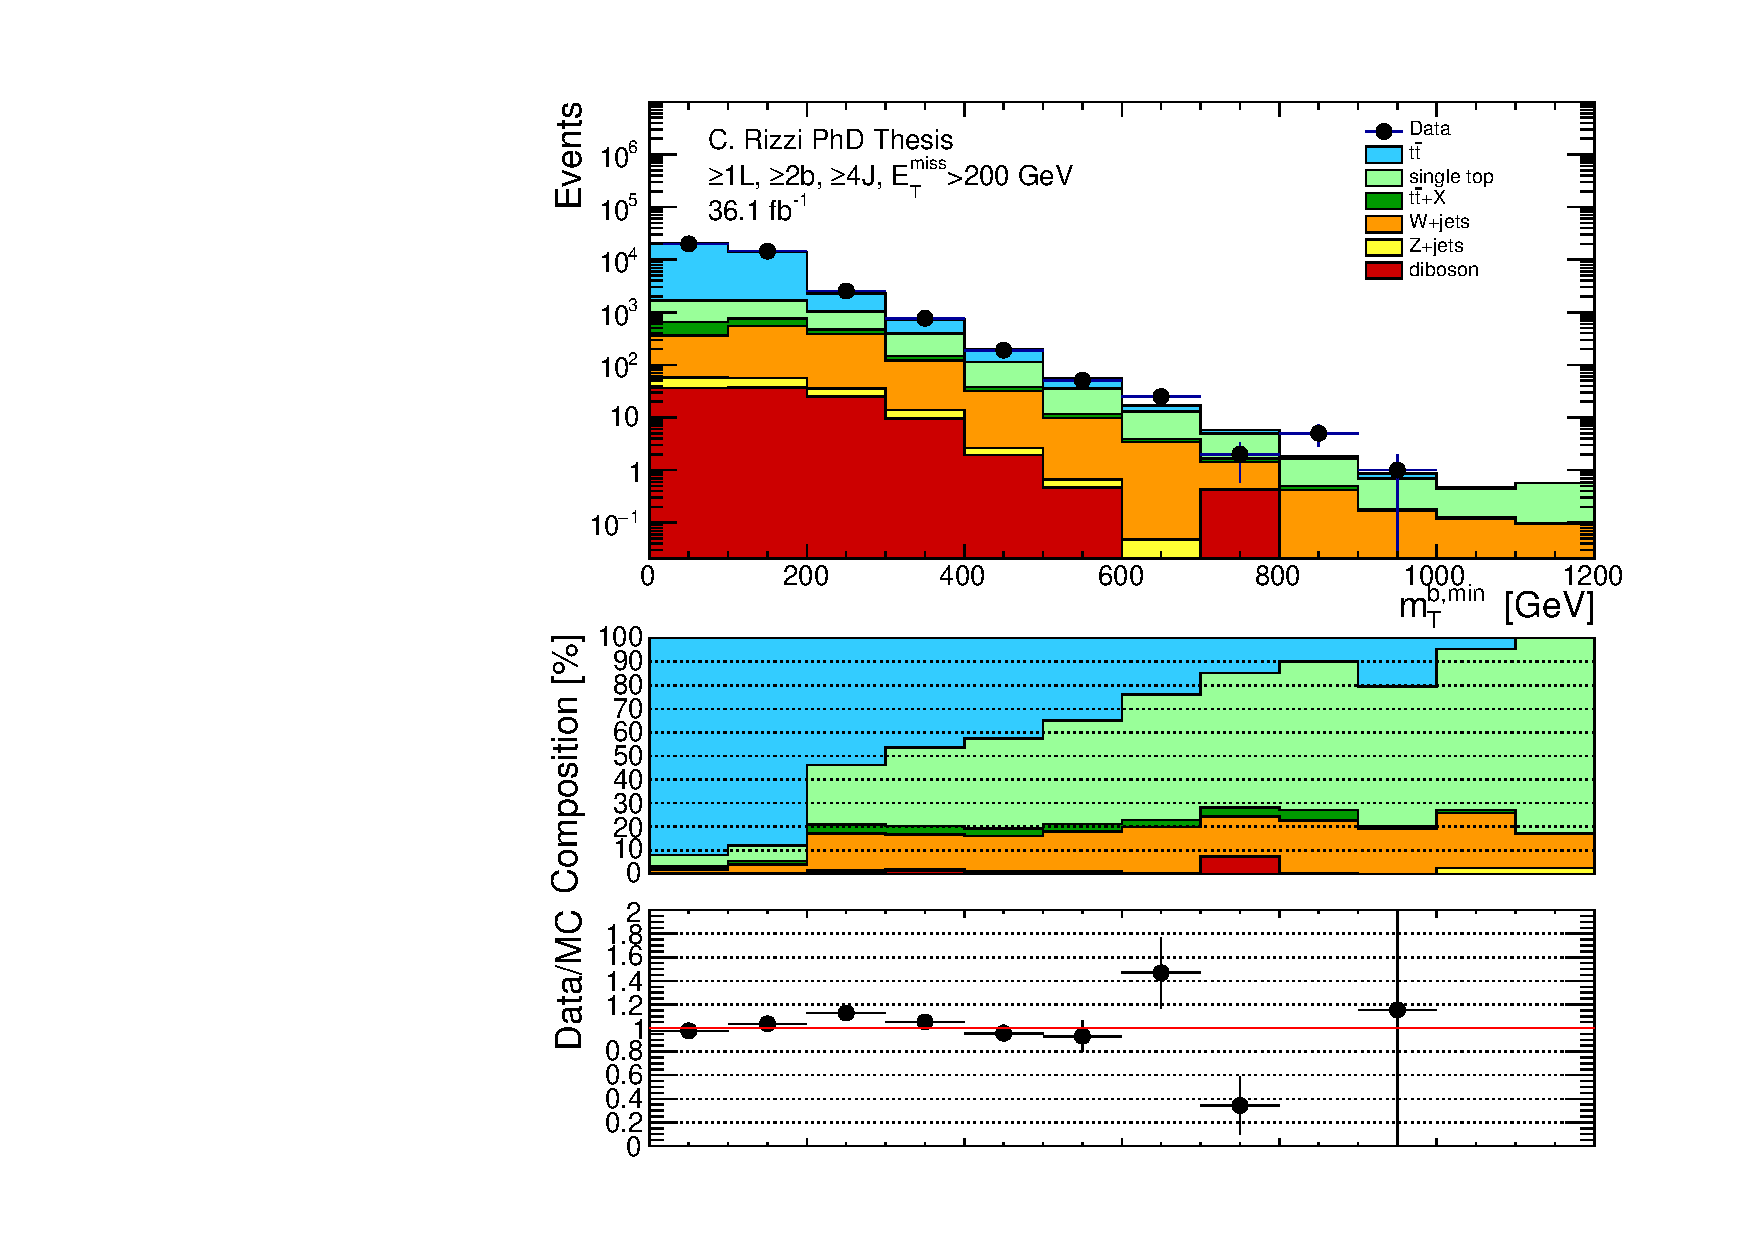
\includegraphics[width=0.45\textwidth]{figures/strong_prod/data_mc/1L_2bin_rw/data_mc_mTb_min.pdf}
\label{fig:strong:datamc1L:mTb_min}}
\caption{Data-MC comparison in the 1-lepton preselection, after applying the kinematic reweighting.
}
\label{fig:strong:datamc1L_a}
\end{figure*}

\begin{figure*}[htbp]
\centering 
\subfigure[\njet]{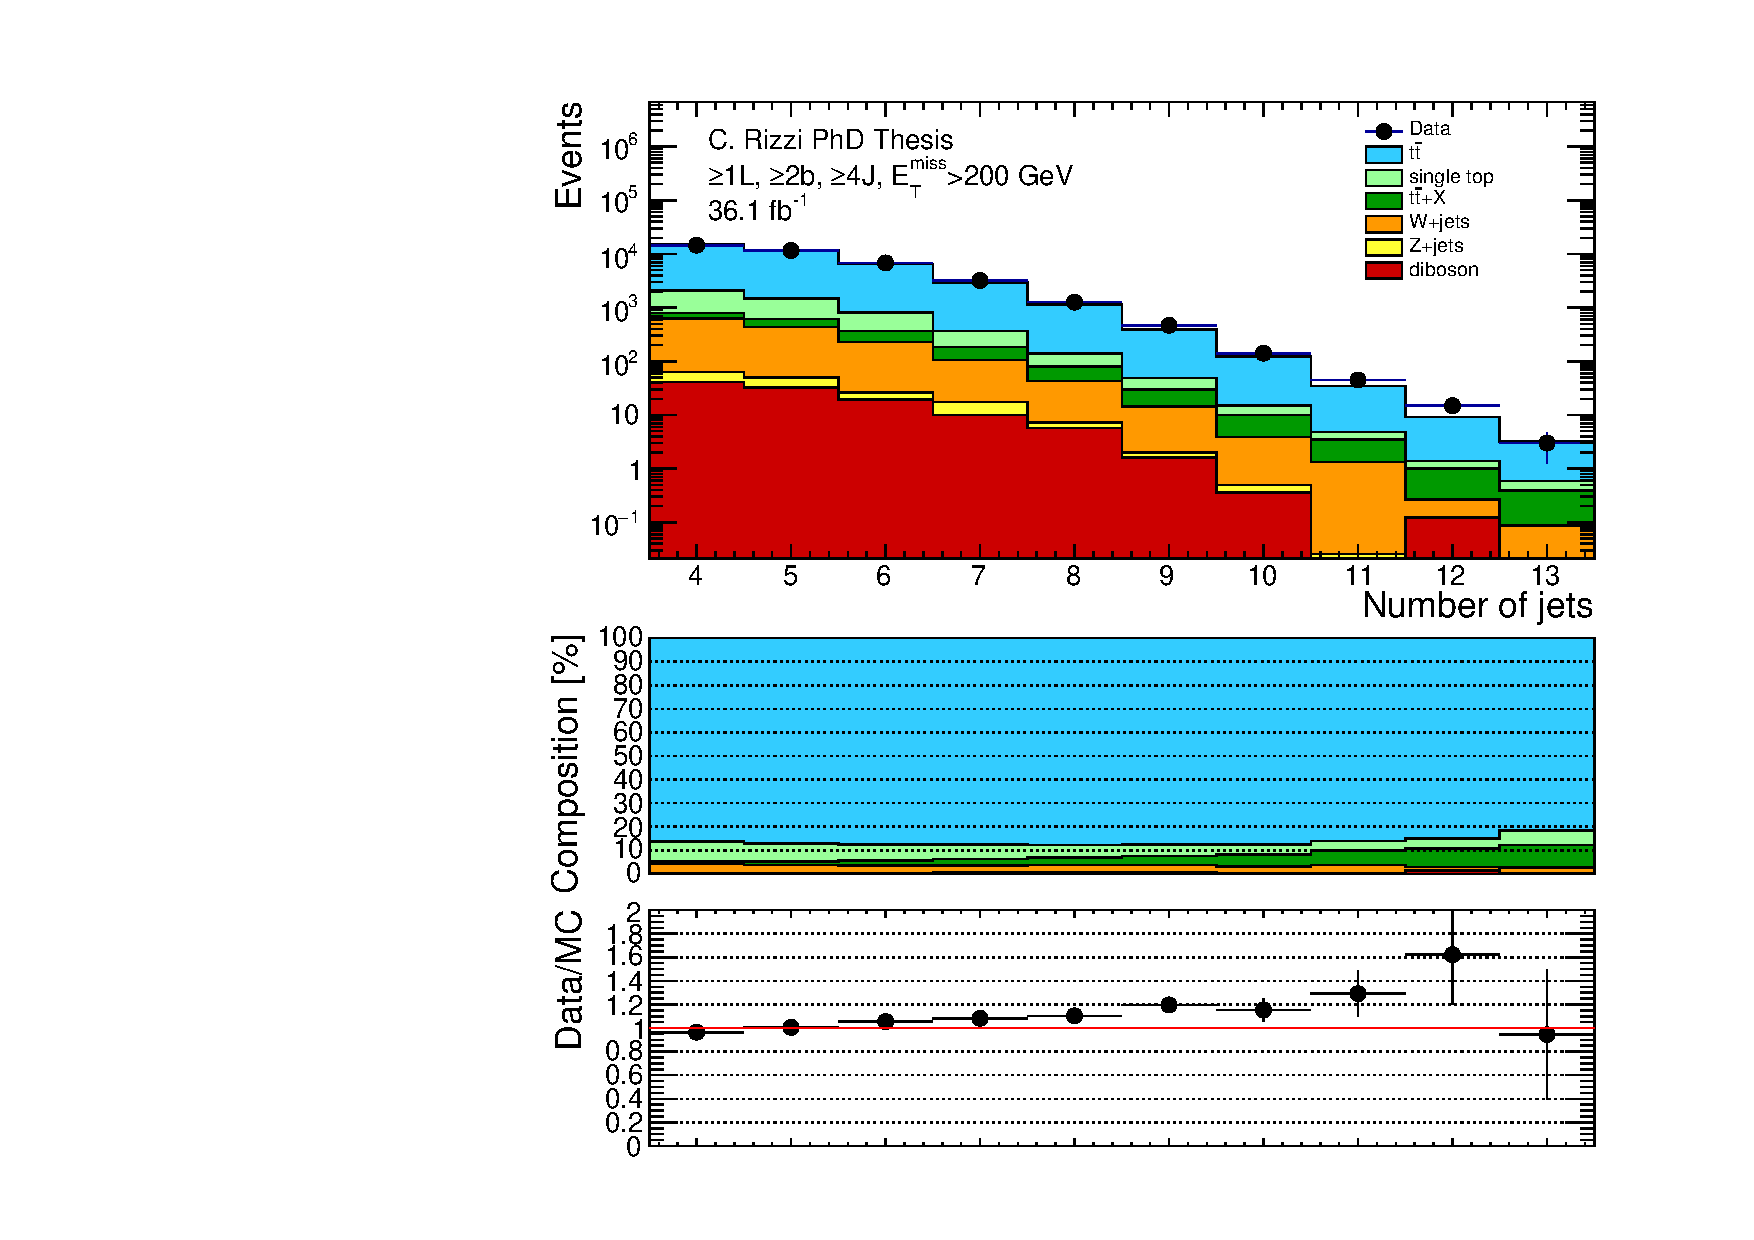
\includegraphics[width=0.45\textwidth]{figures/strong_prod/data_mc/1L_2bin_rw/data_mc_jets_n.pdf}
\label{fig:strong:datamc1L:jets_n}}
\subfigure[\nbjet]{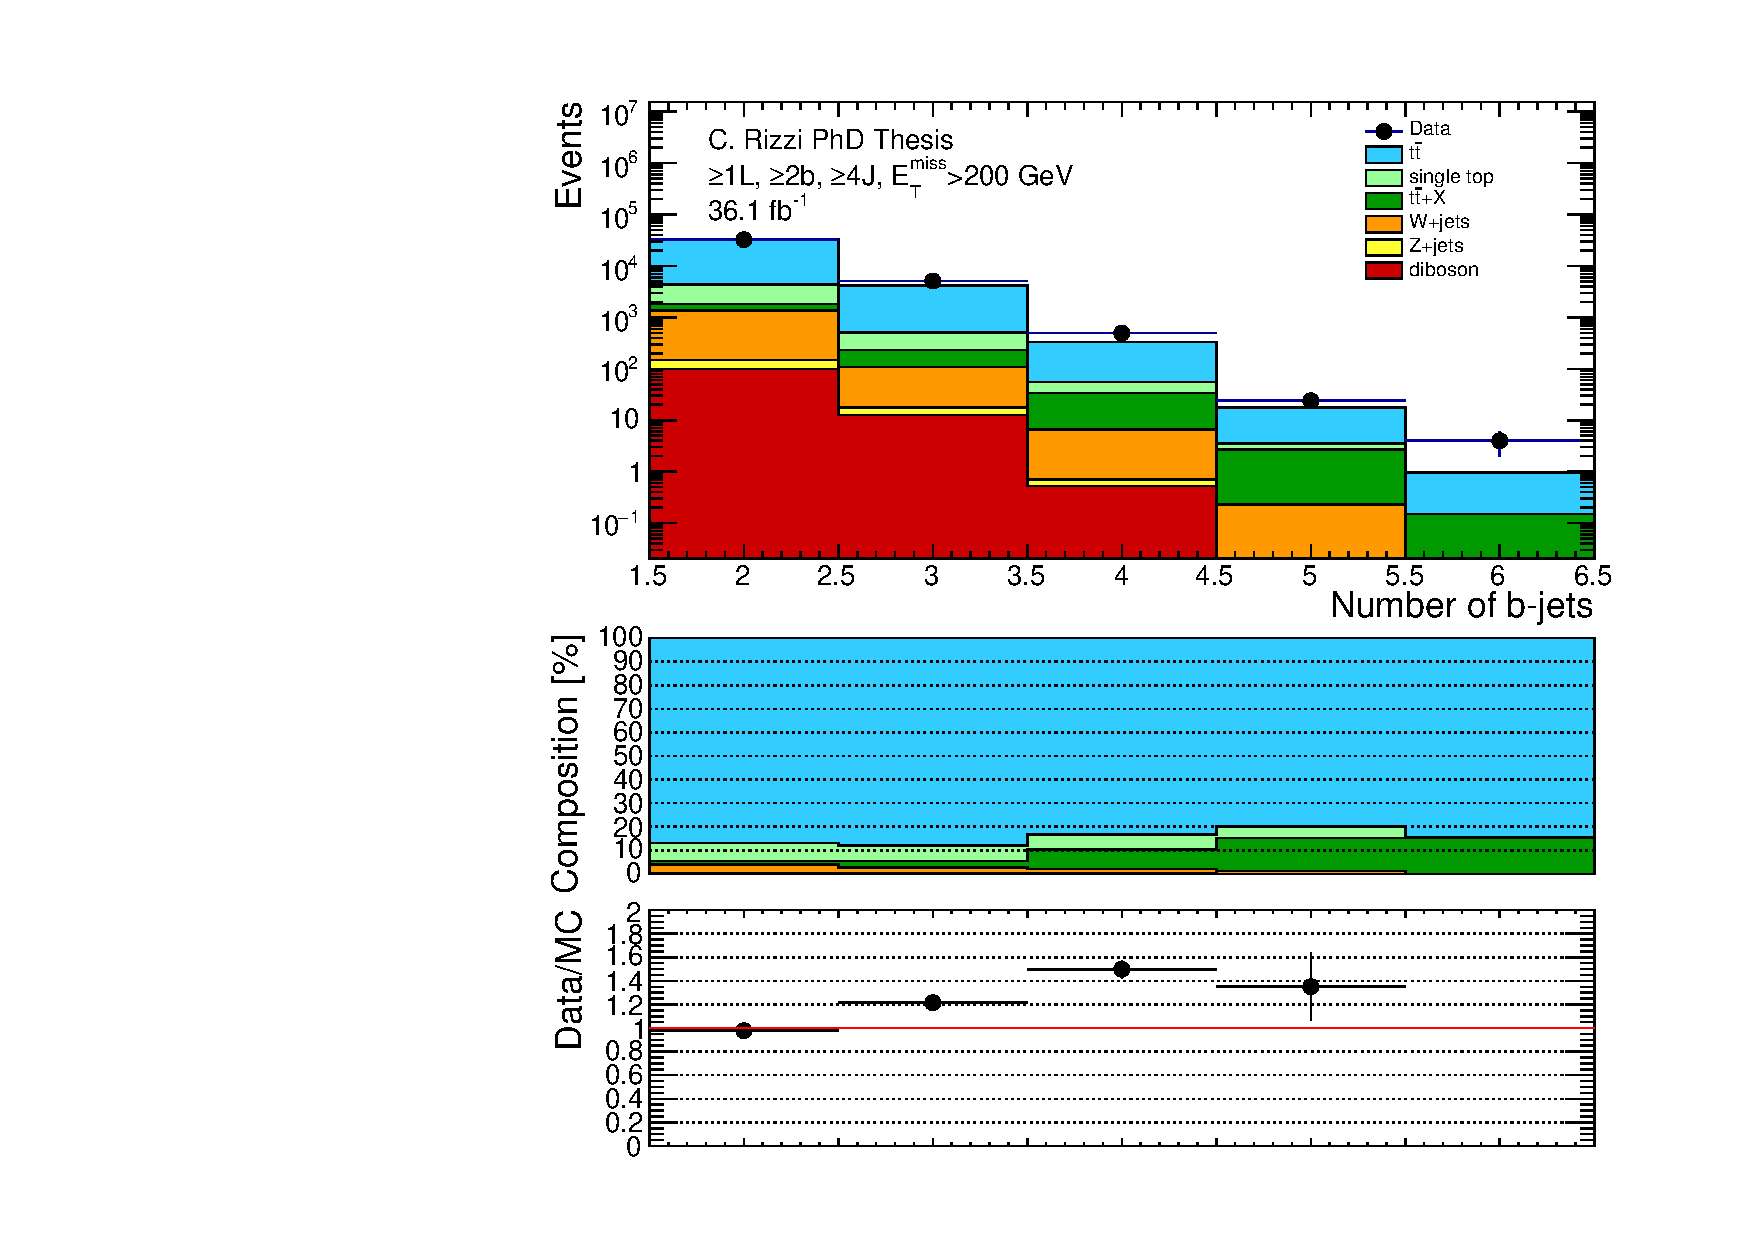
\includegraphics[width=0.45\textwidth]{figures/strong_prod/data_mc/1L_2bin_rw/data_mc_bjets_n.pdf}
\label{fig:strong:datamc1L:bjets_n}}\\
\subfigure[\pt jet$_1$]{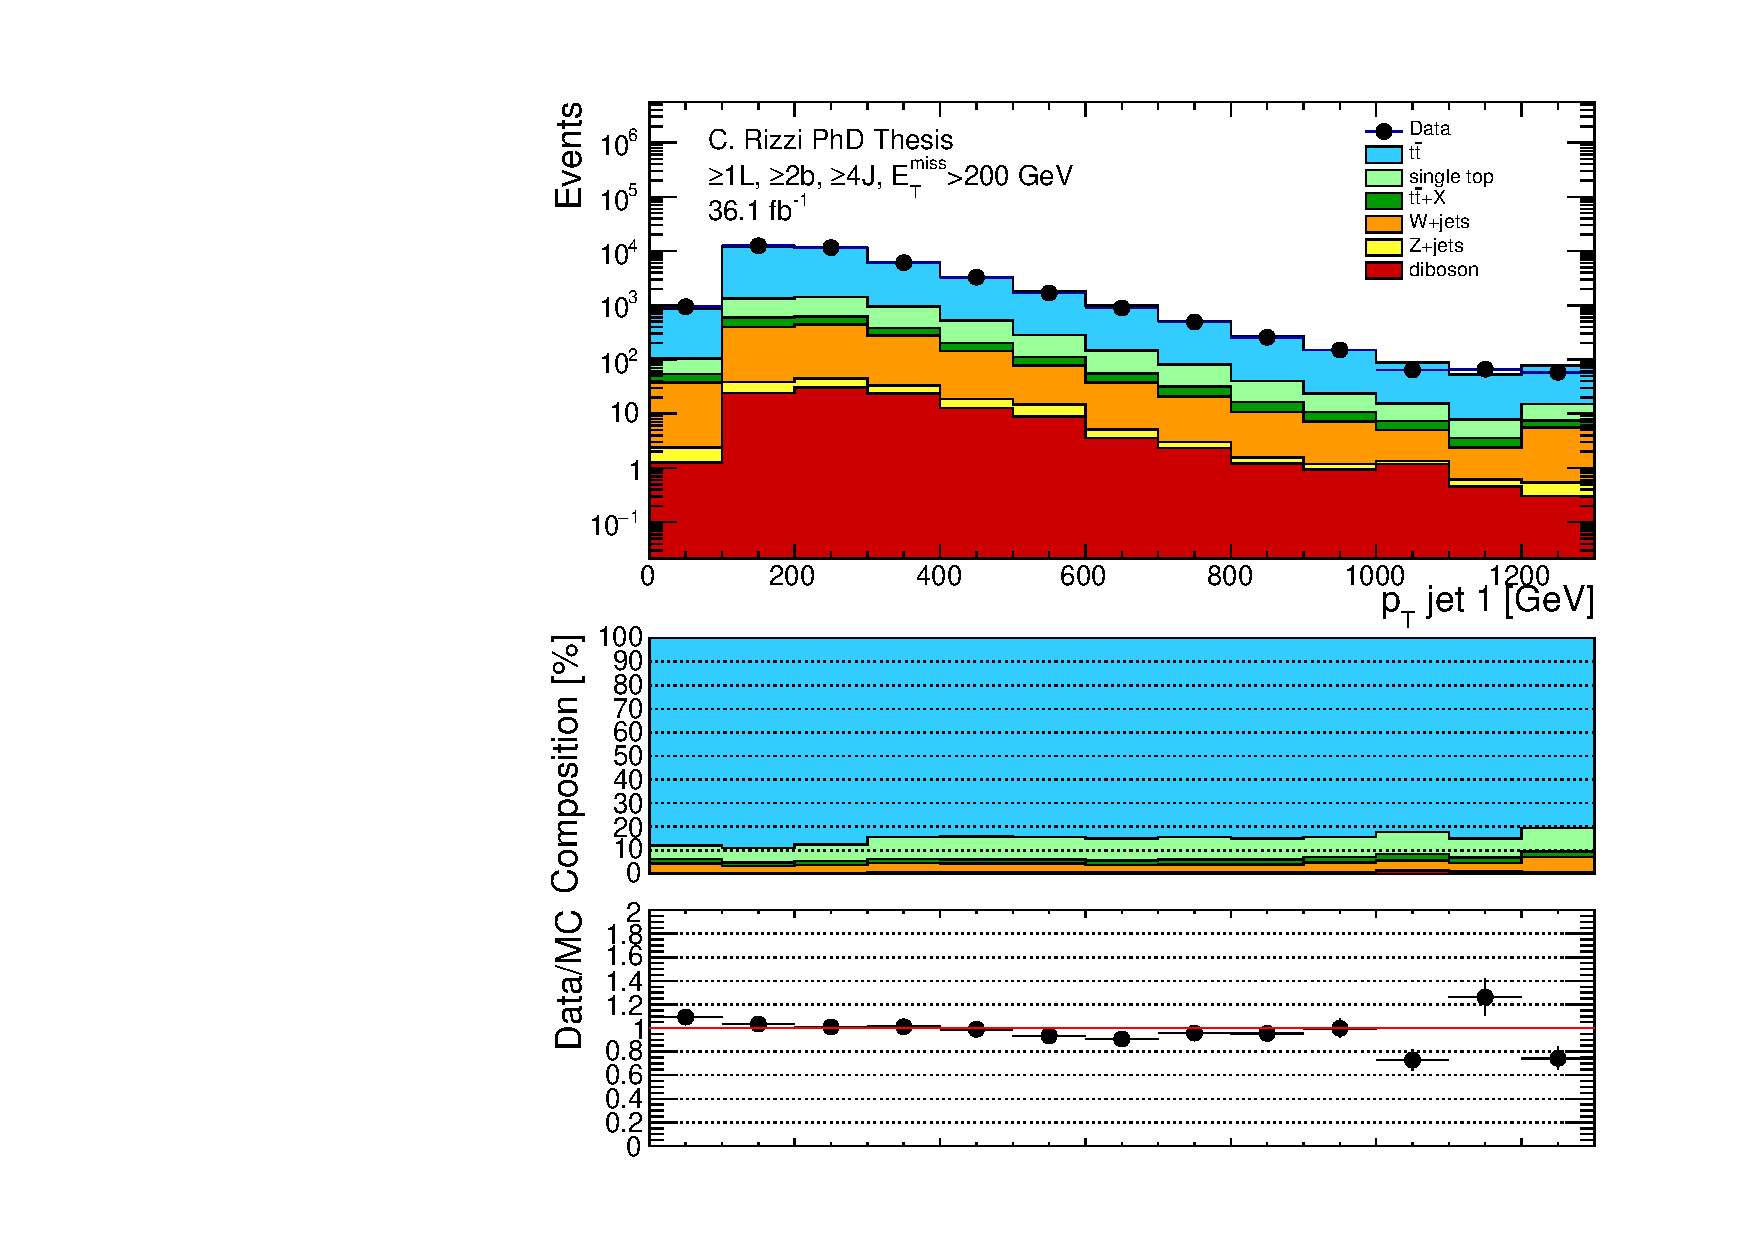
\includegraphics[width=0.45\textwidth]{figures/strong_prod/data_mc/1L_2bin_rw/data_mc_pt_jet_1.pdf}
\label{fig:strong:datamc1L:pt_jet_1}}
\subfigure[\pt jet$_2$]{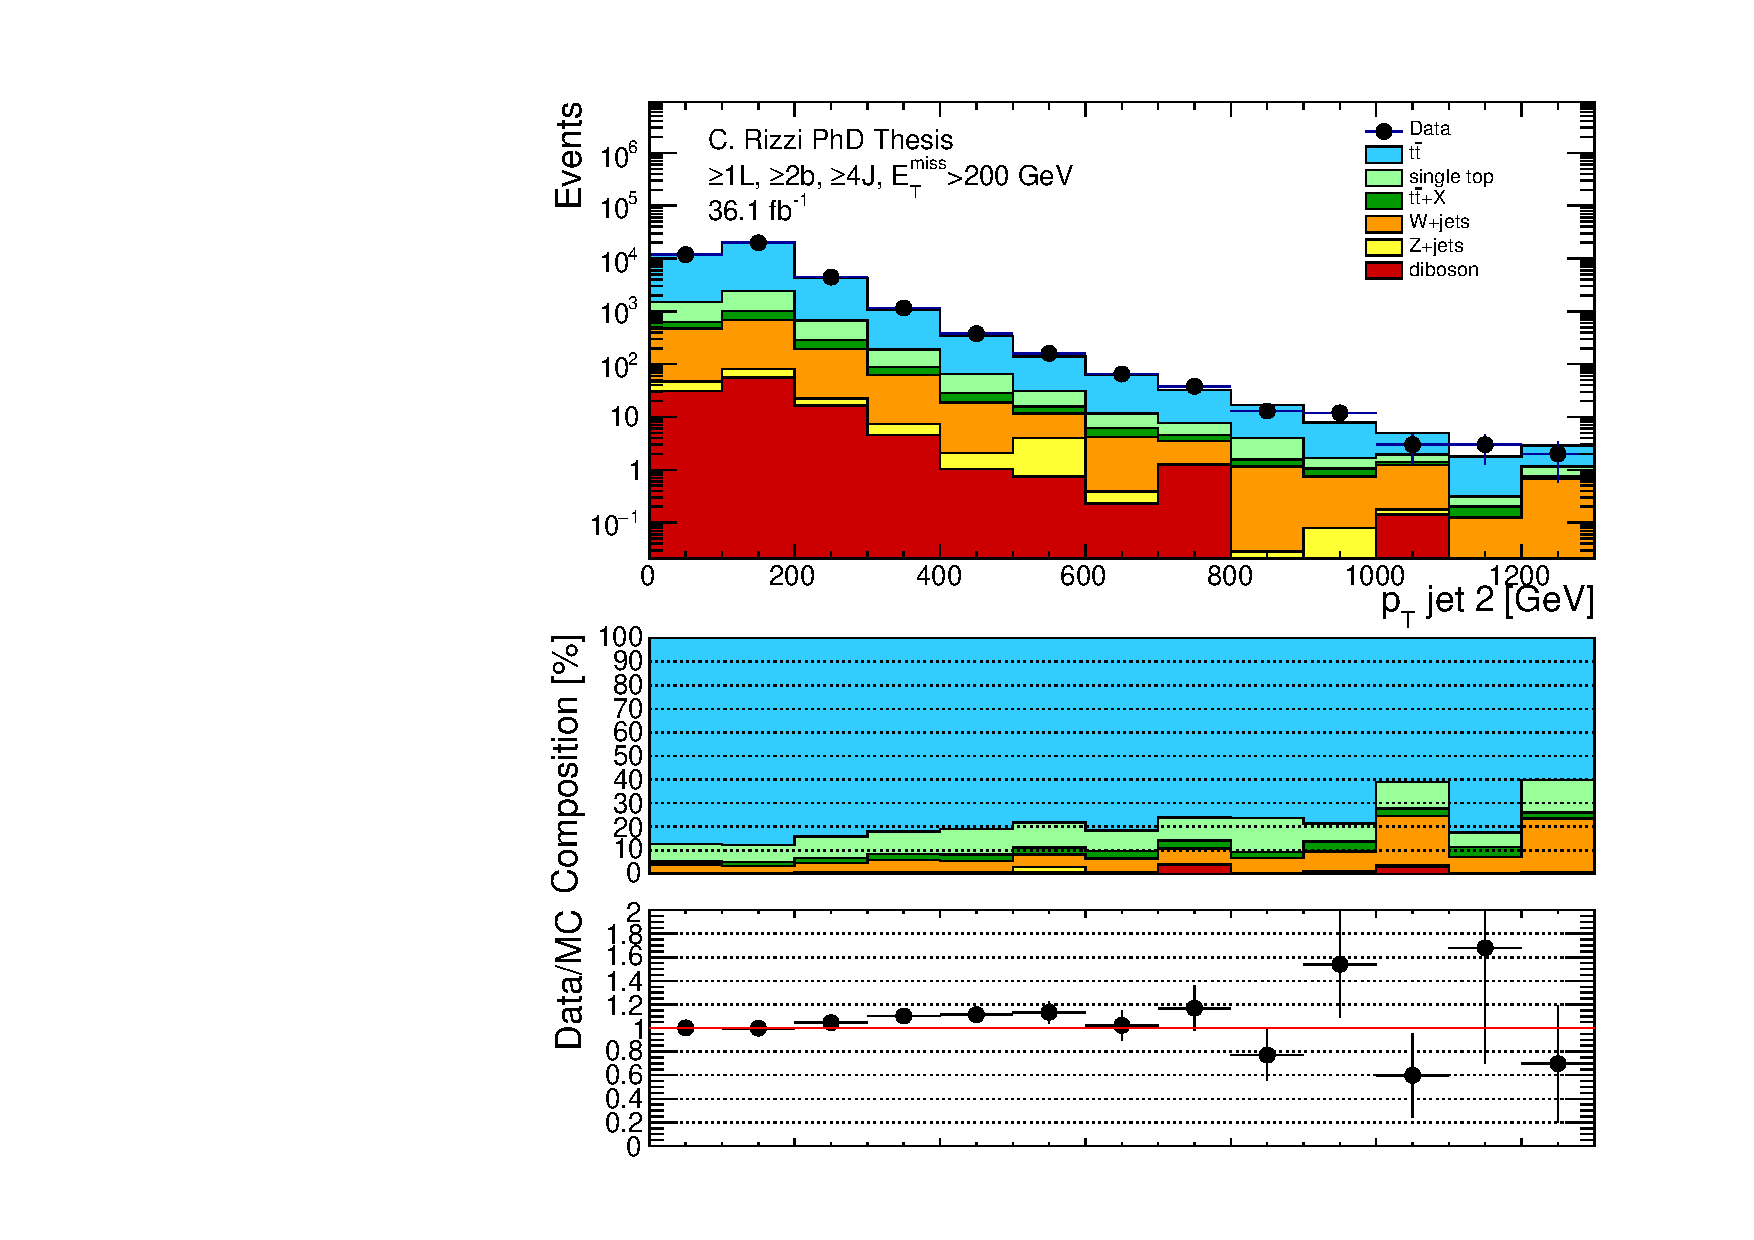
\includegraphics[width=0.45\textwidth]{figures/strong_prod/data_mc/1L_2bin_rw/data_mc_pt_jet_2.pdf}
\label{fig:strong:datamc1L:pt_jet_2}}\\
\subfigure[\pt lep$_1$]{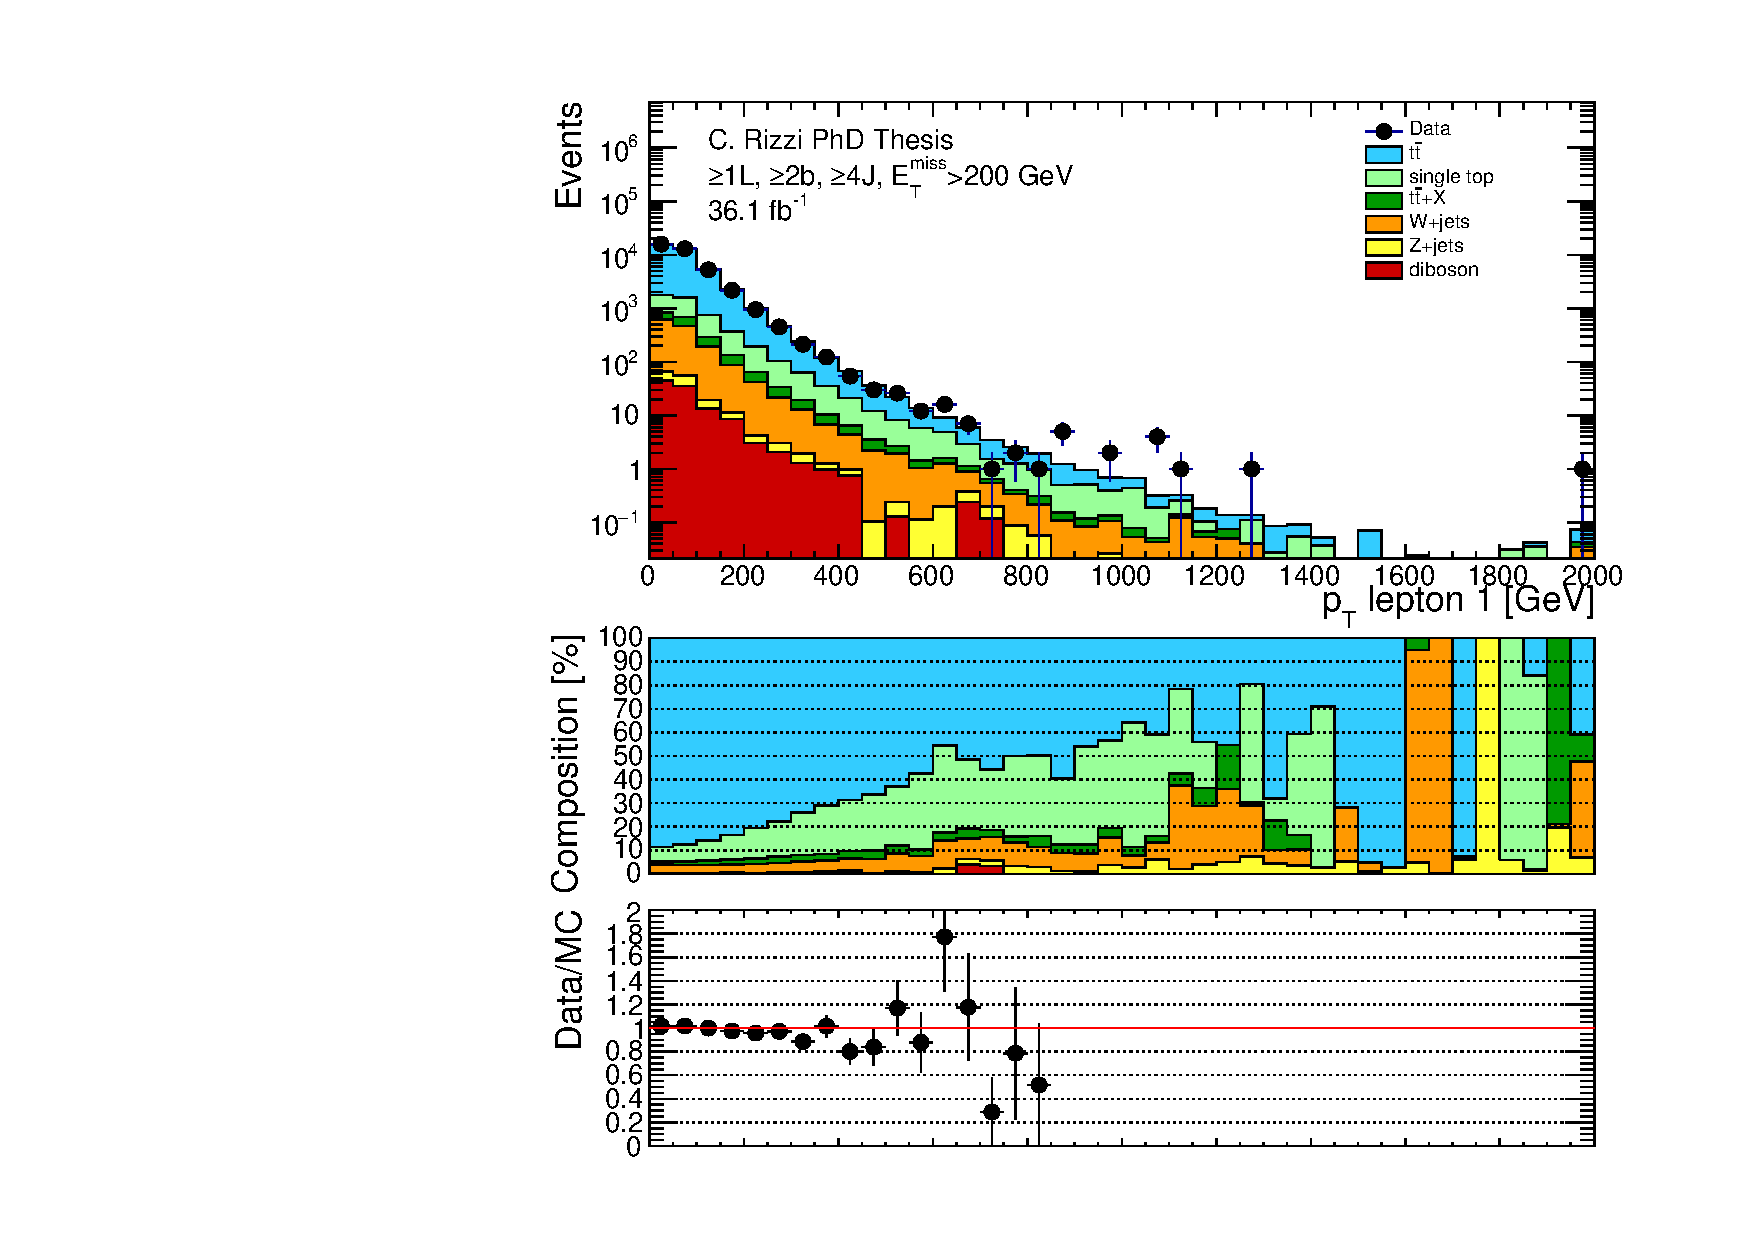
\includegraphics[width=0.45\textwidth]{figures/strong_prod/data_mc/1L_2bin_rw/data_mc_pt_lep_1.pdf}
\label{fig:strong:datamc1L:ptlep1}}
\subfigure[\pt b-jet$_1$]{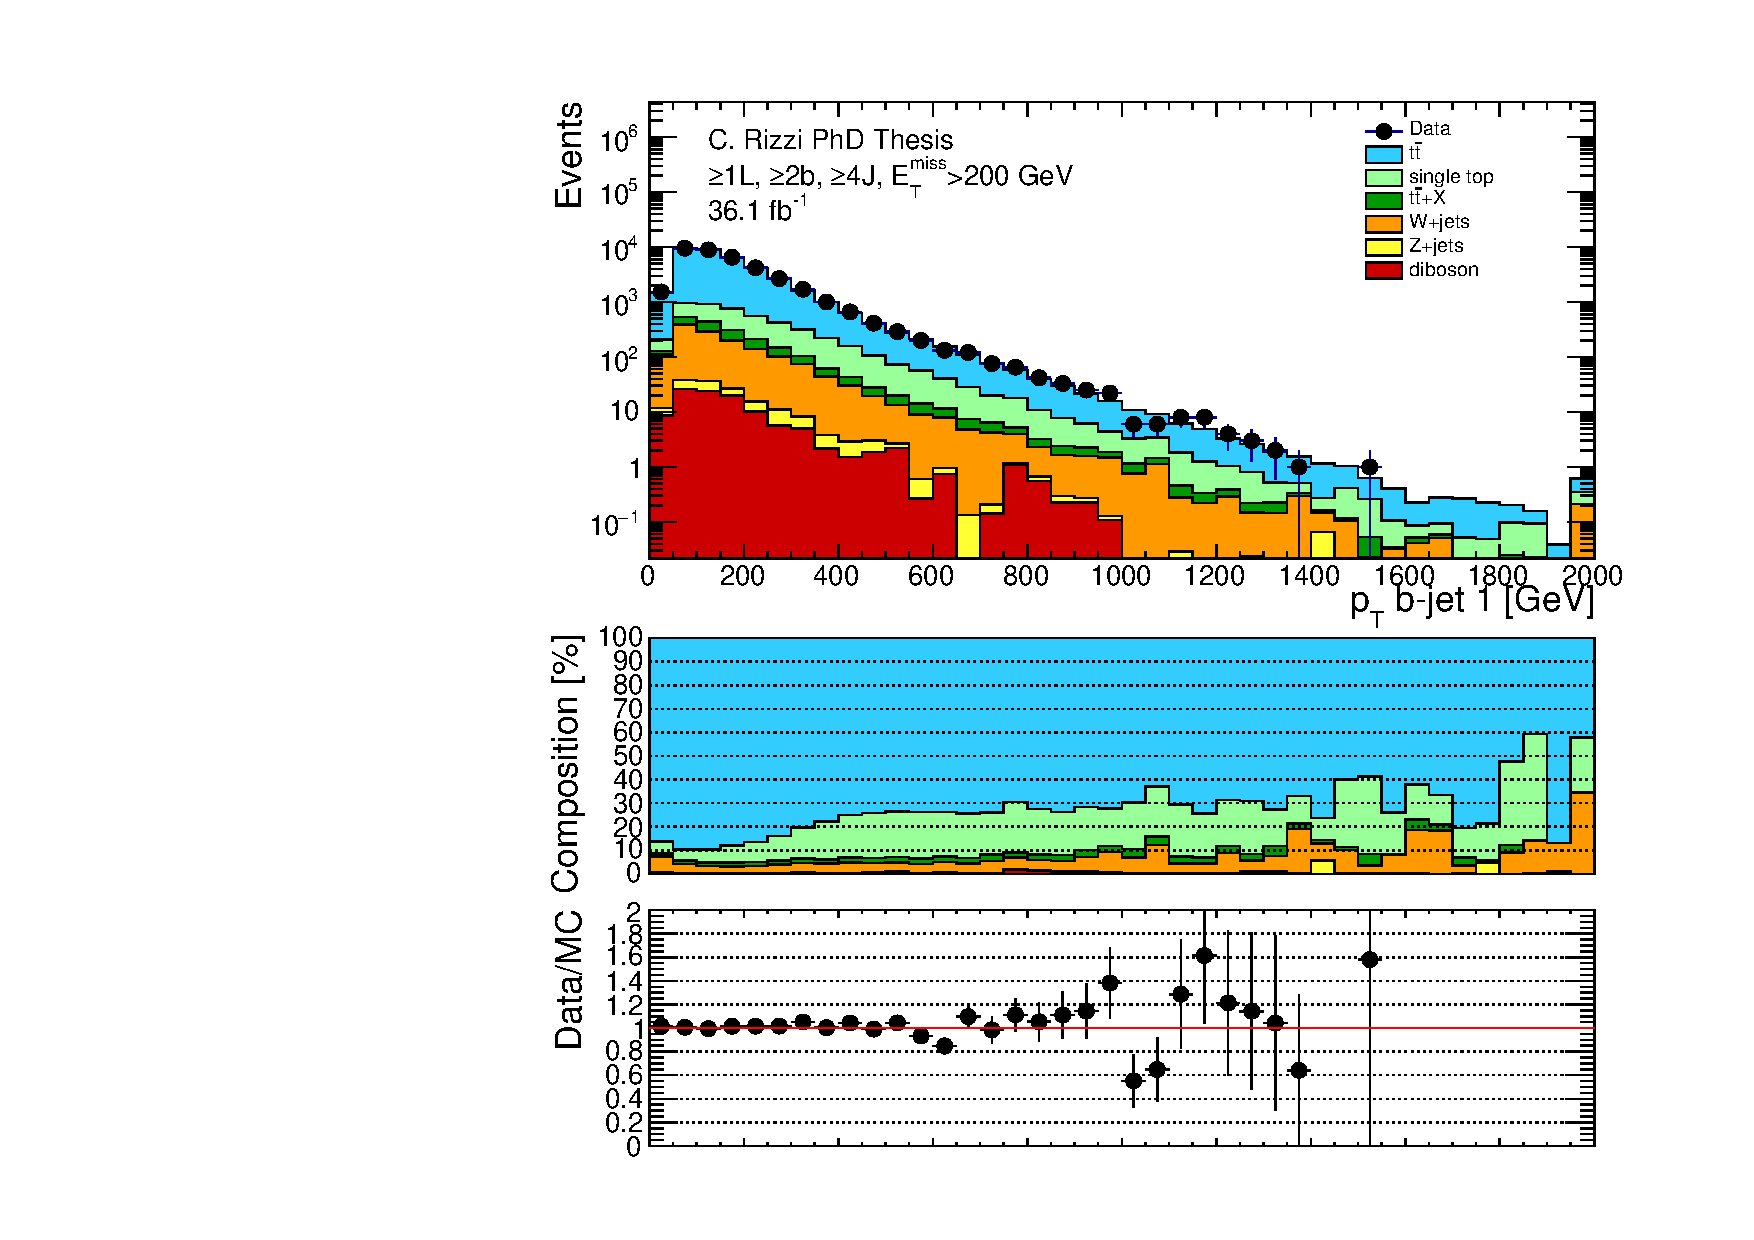
\includegraphics[width=0.45\textwidth]{figures/strong_prod/data_mc/1L_2bin_rw/data_mc_pt_bjet_1.pdf}
\label{fig:strong:datamc1L:pt_bjet_1}}
\caption{Data-MC comparison in the 1-lepton preselection, after applying the kinematic reweighting.
}
\label{fig:strong:datamc1L_b}
\end{figure*}

\begin{figure*}[htbp]
\centering 
\subfigure[\meff]{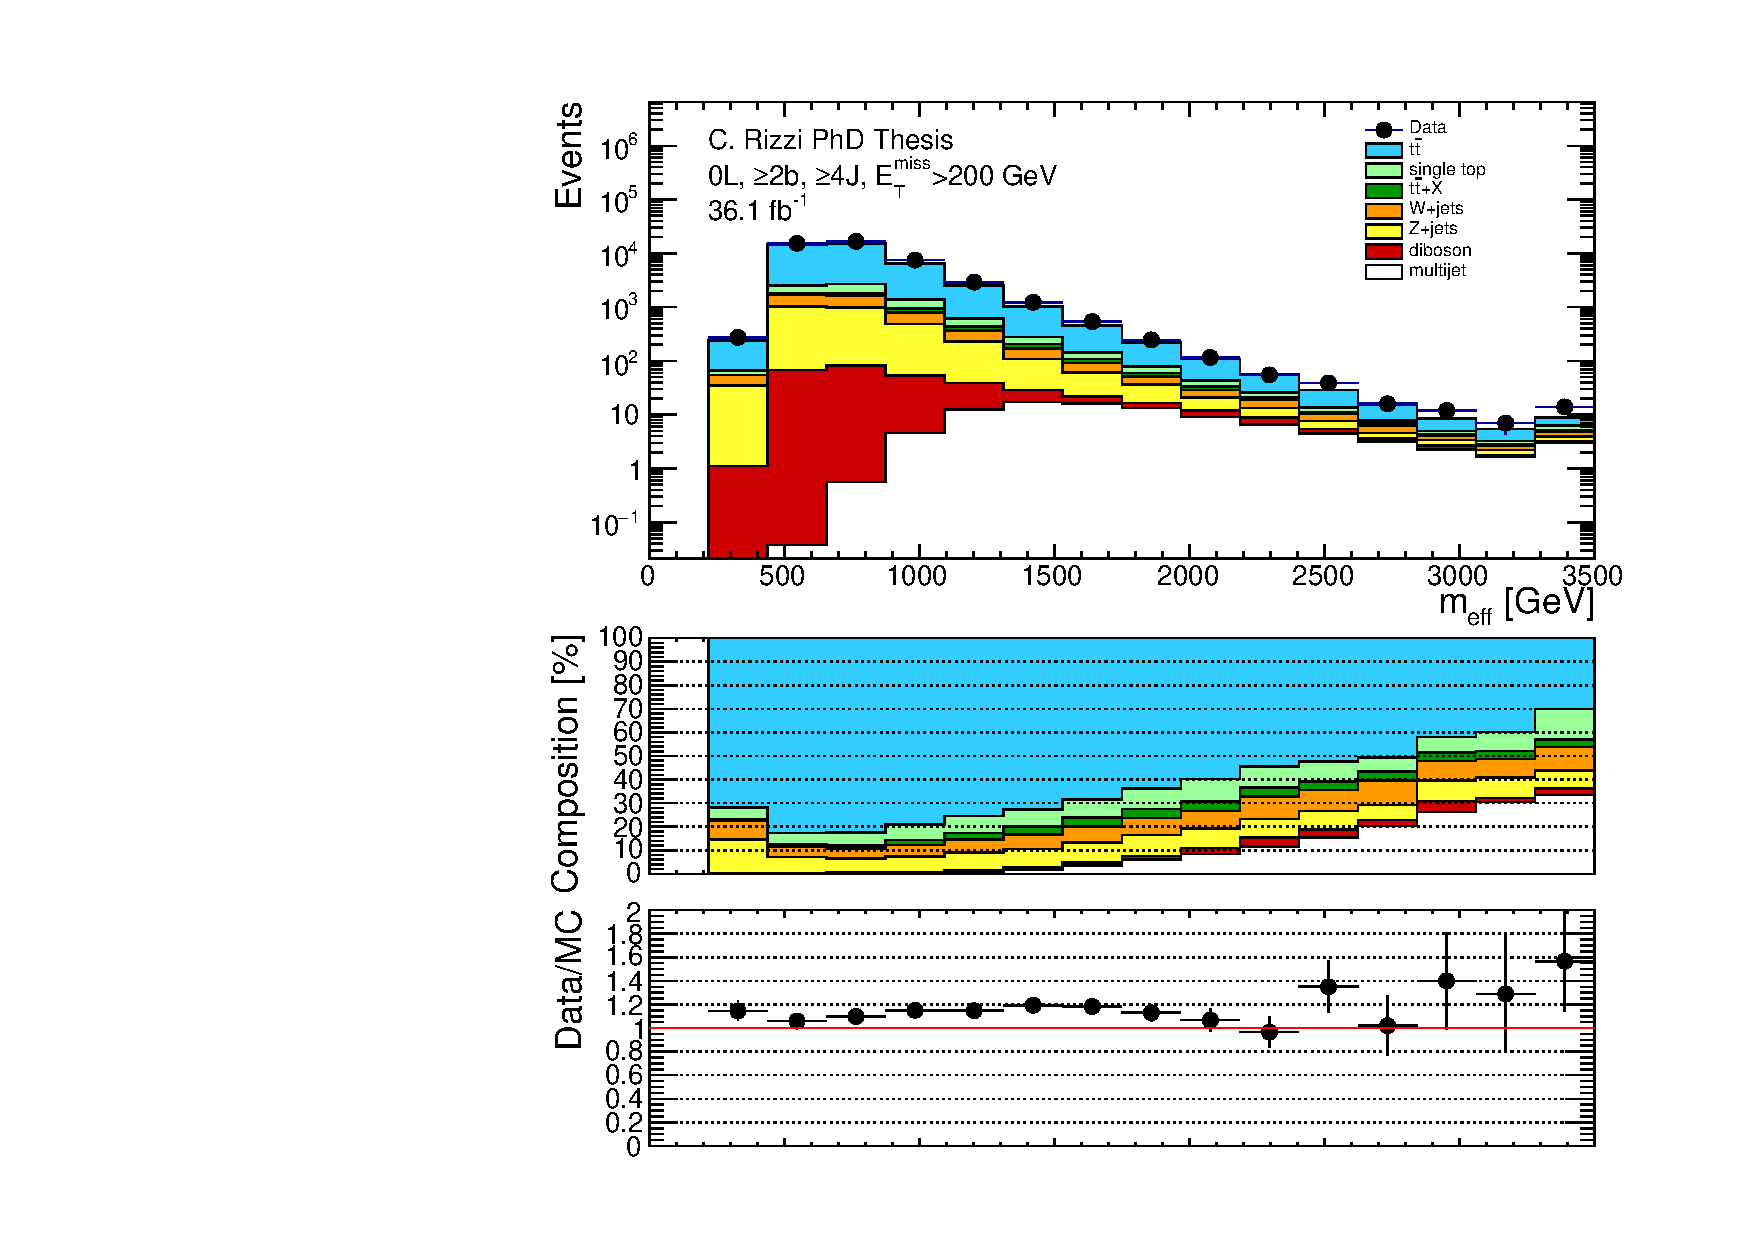
\includegraphics[width=0.45\textwidth]{figures/strong_prod/data_mc/0L_2bin/data_mc_meff_incl.pdf}
\label{fig:strong:datamc0L:meff_incl}}
\subfigure[\mjsum]{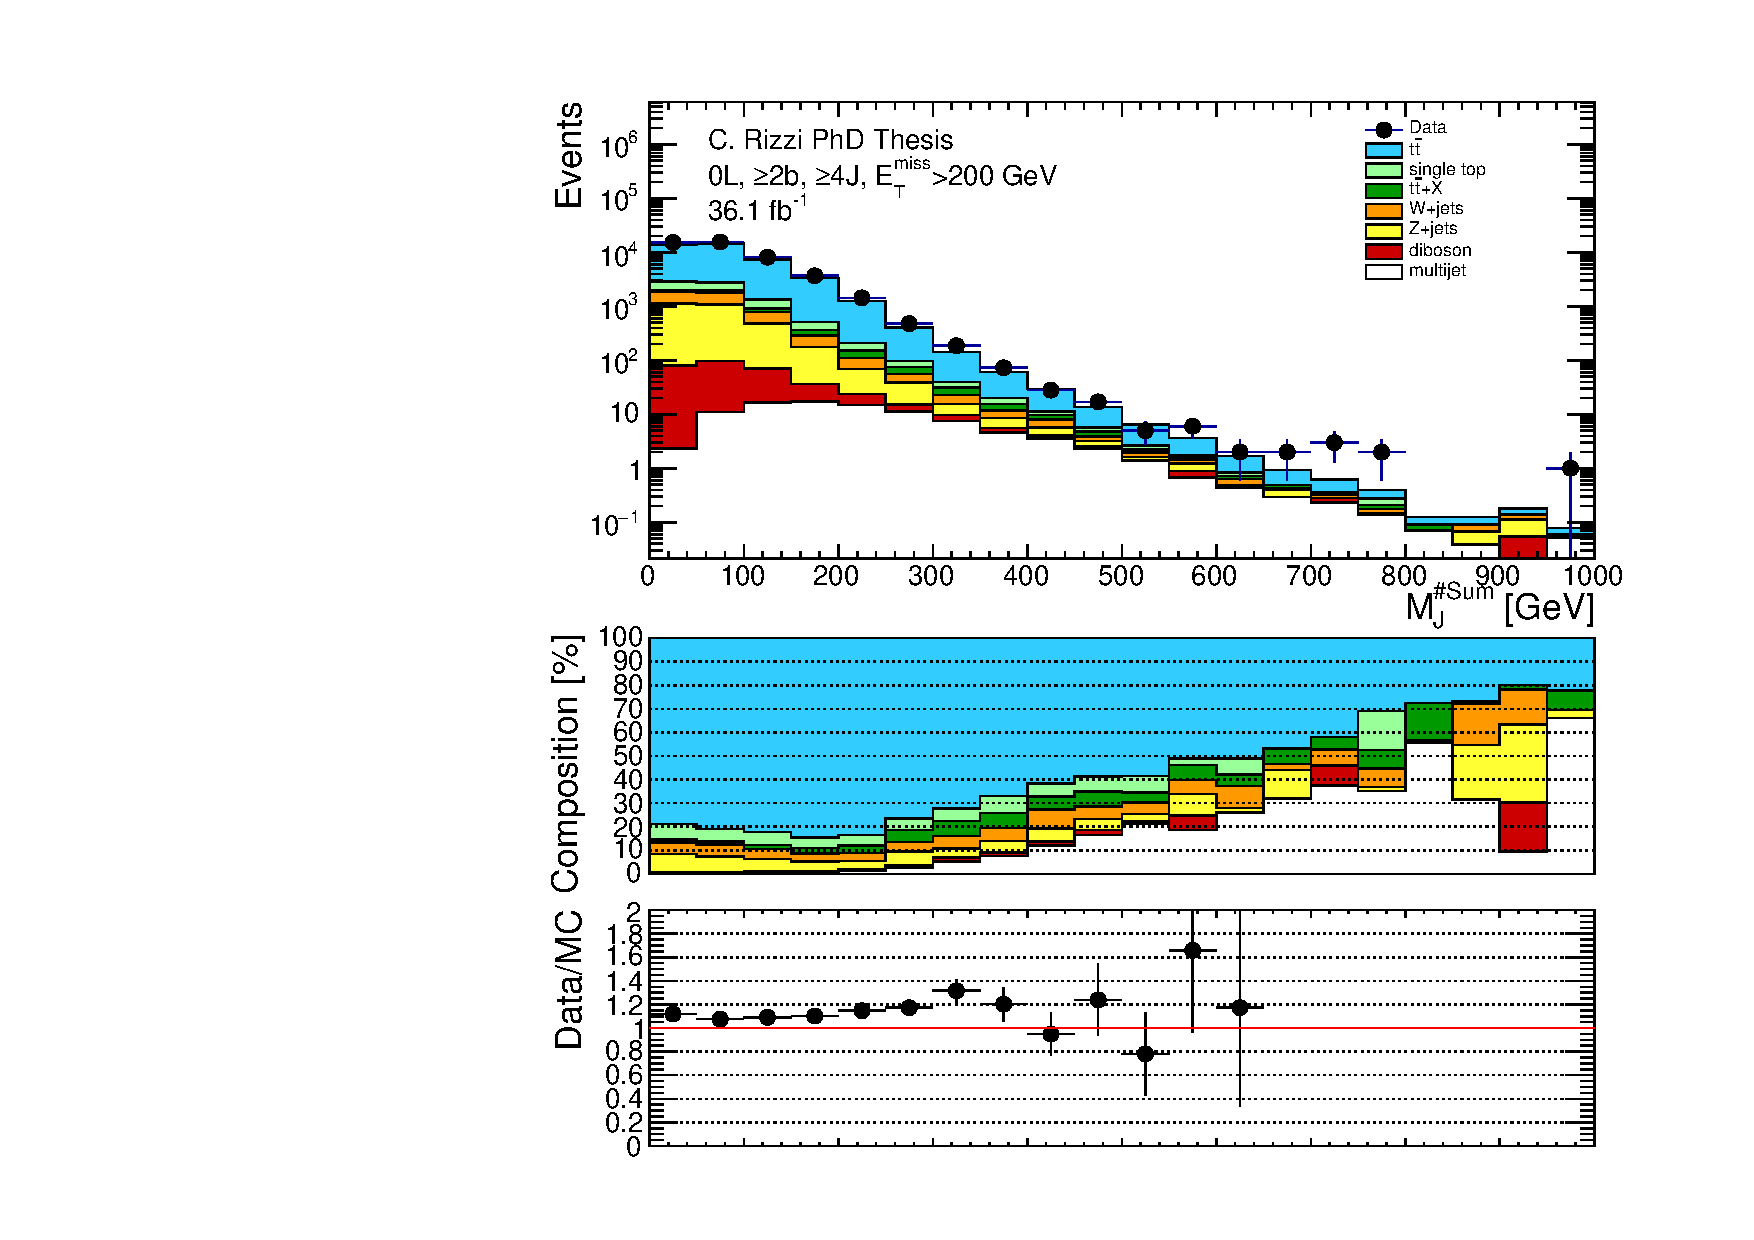
\includegraphics[width=0.45\textwidth]{figures/strong_prod/data_mc/0L_2bin/data_mc_MJSum_rc_r08pt10.pdf}
\label{fig:strong:datamc0L:MJSum_rc_r08pt10}}\\
\subfigure[\met]{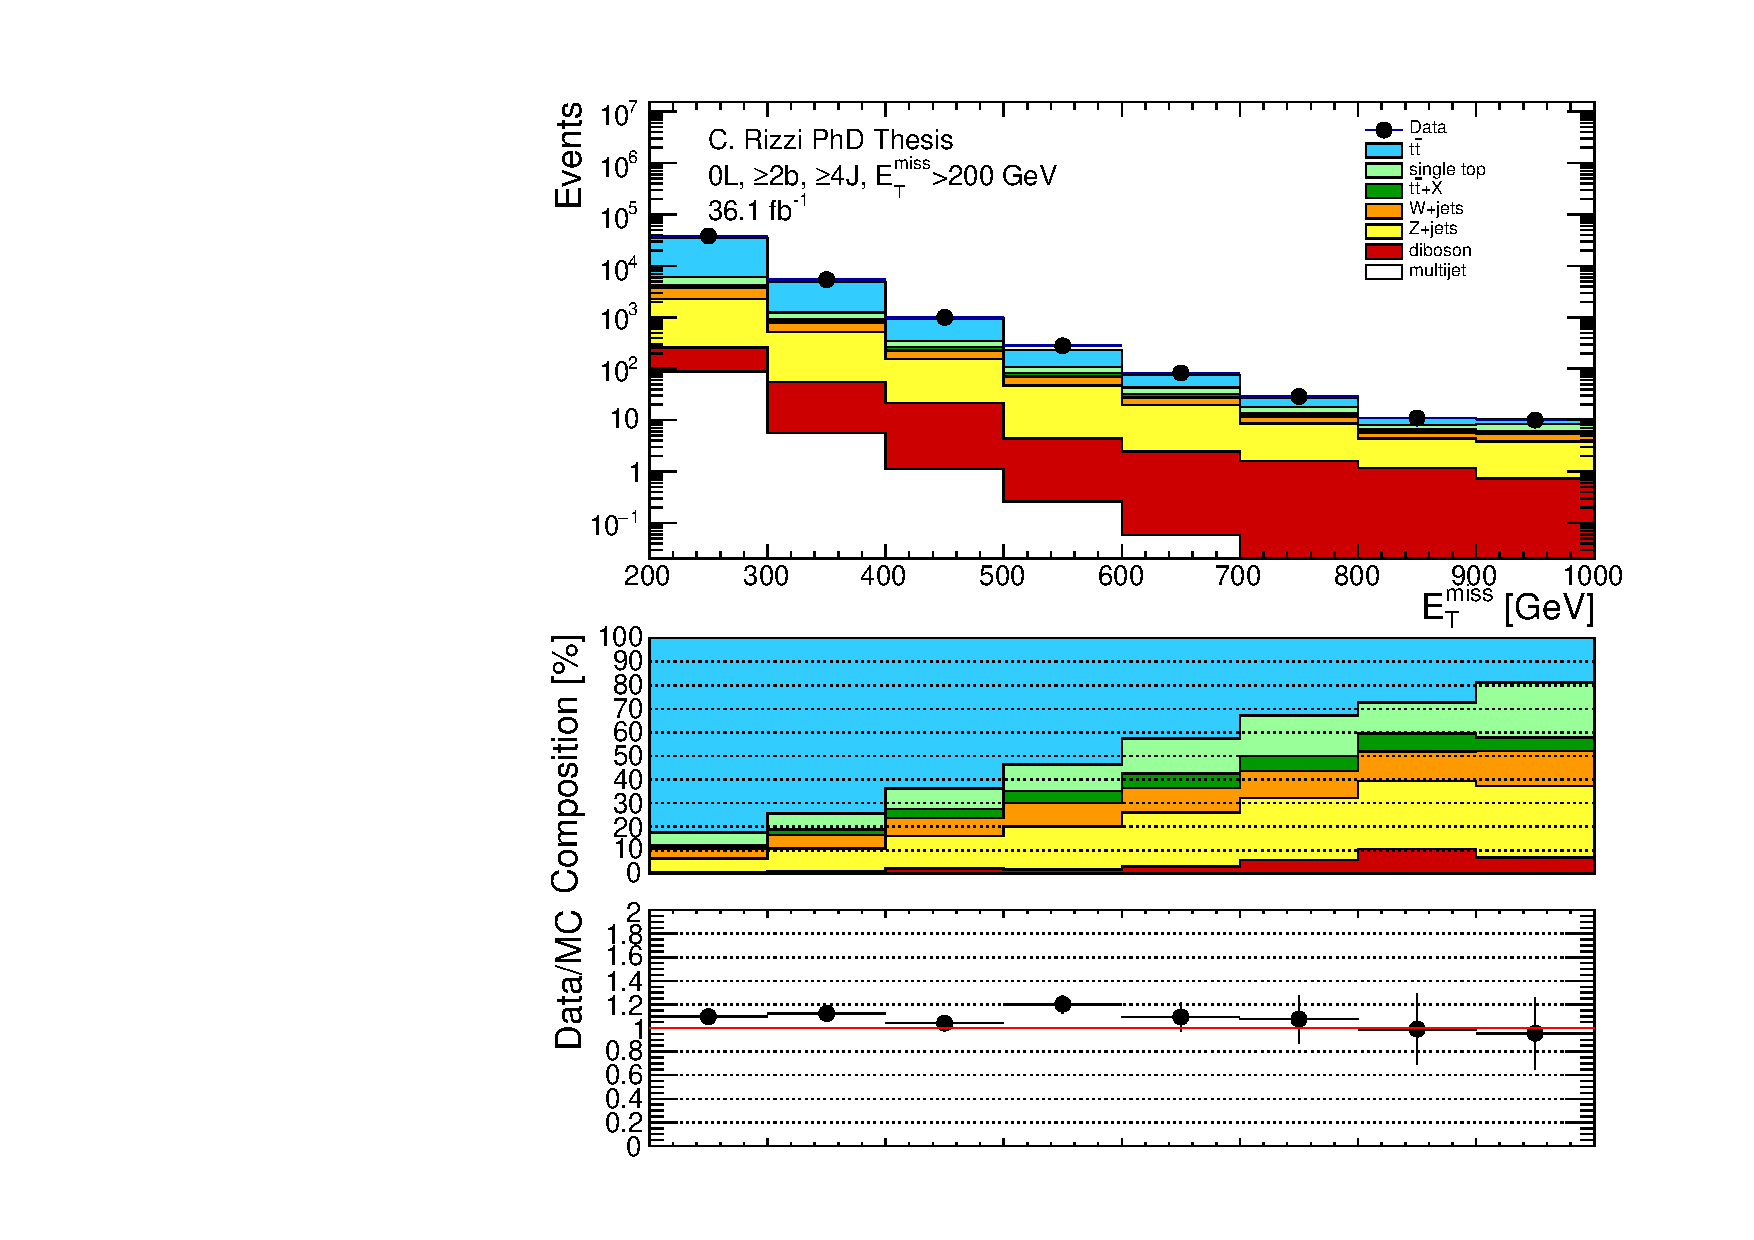
\includegraphics[width=0.45\textwidth]{figures/strong_prod/data_mc/0L_2bin/data_mc_met.pdf}
\label{fig:strong:datamc0L:met}}
\subfigure[$\phi$(\met)]{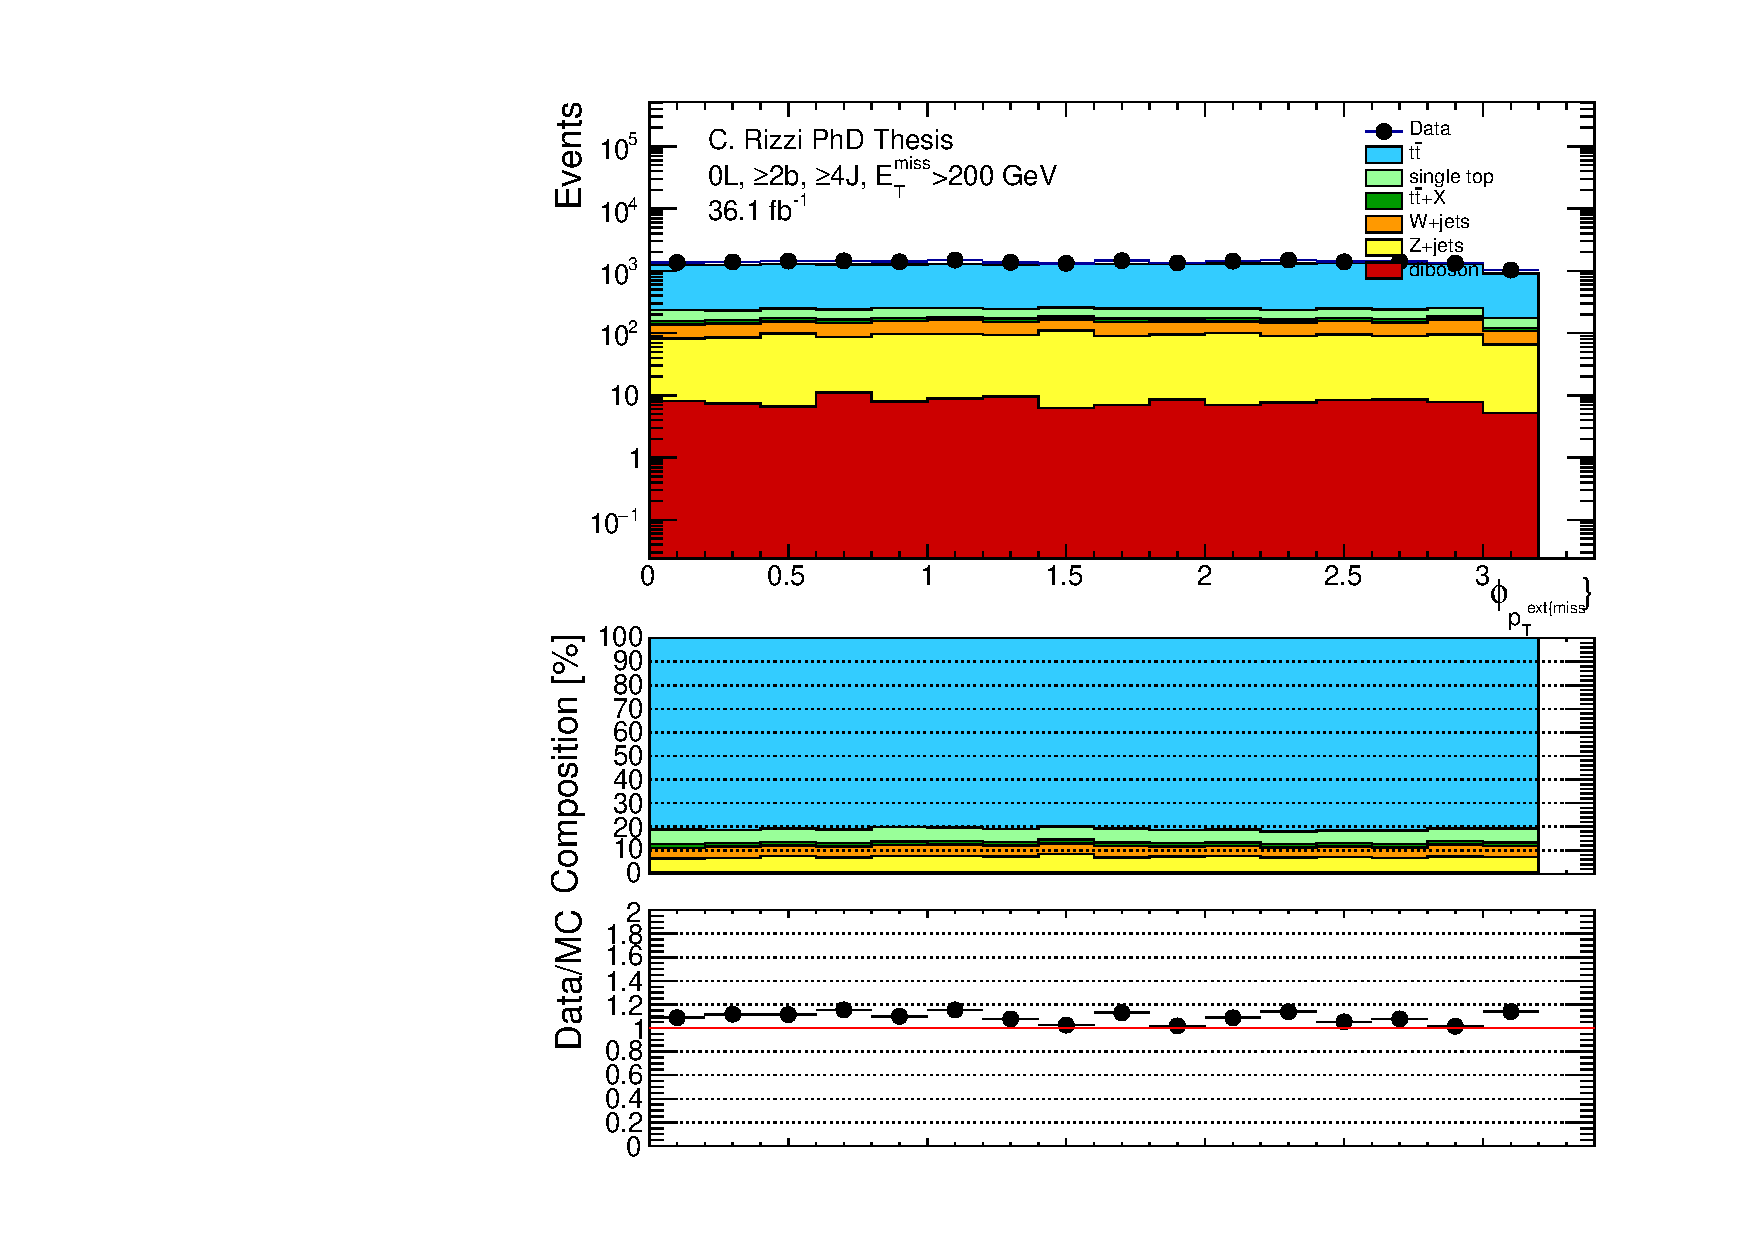
\includegraphics[width=0.45\textwidth]{figures/strong_prod/data_mc/0L_2bin/data_mc_met_phi.pdf}
\label{fig:strong:datamc0L:met_phi}}\\
\subfigure[\mt]{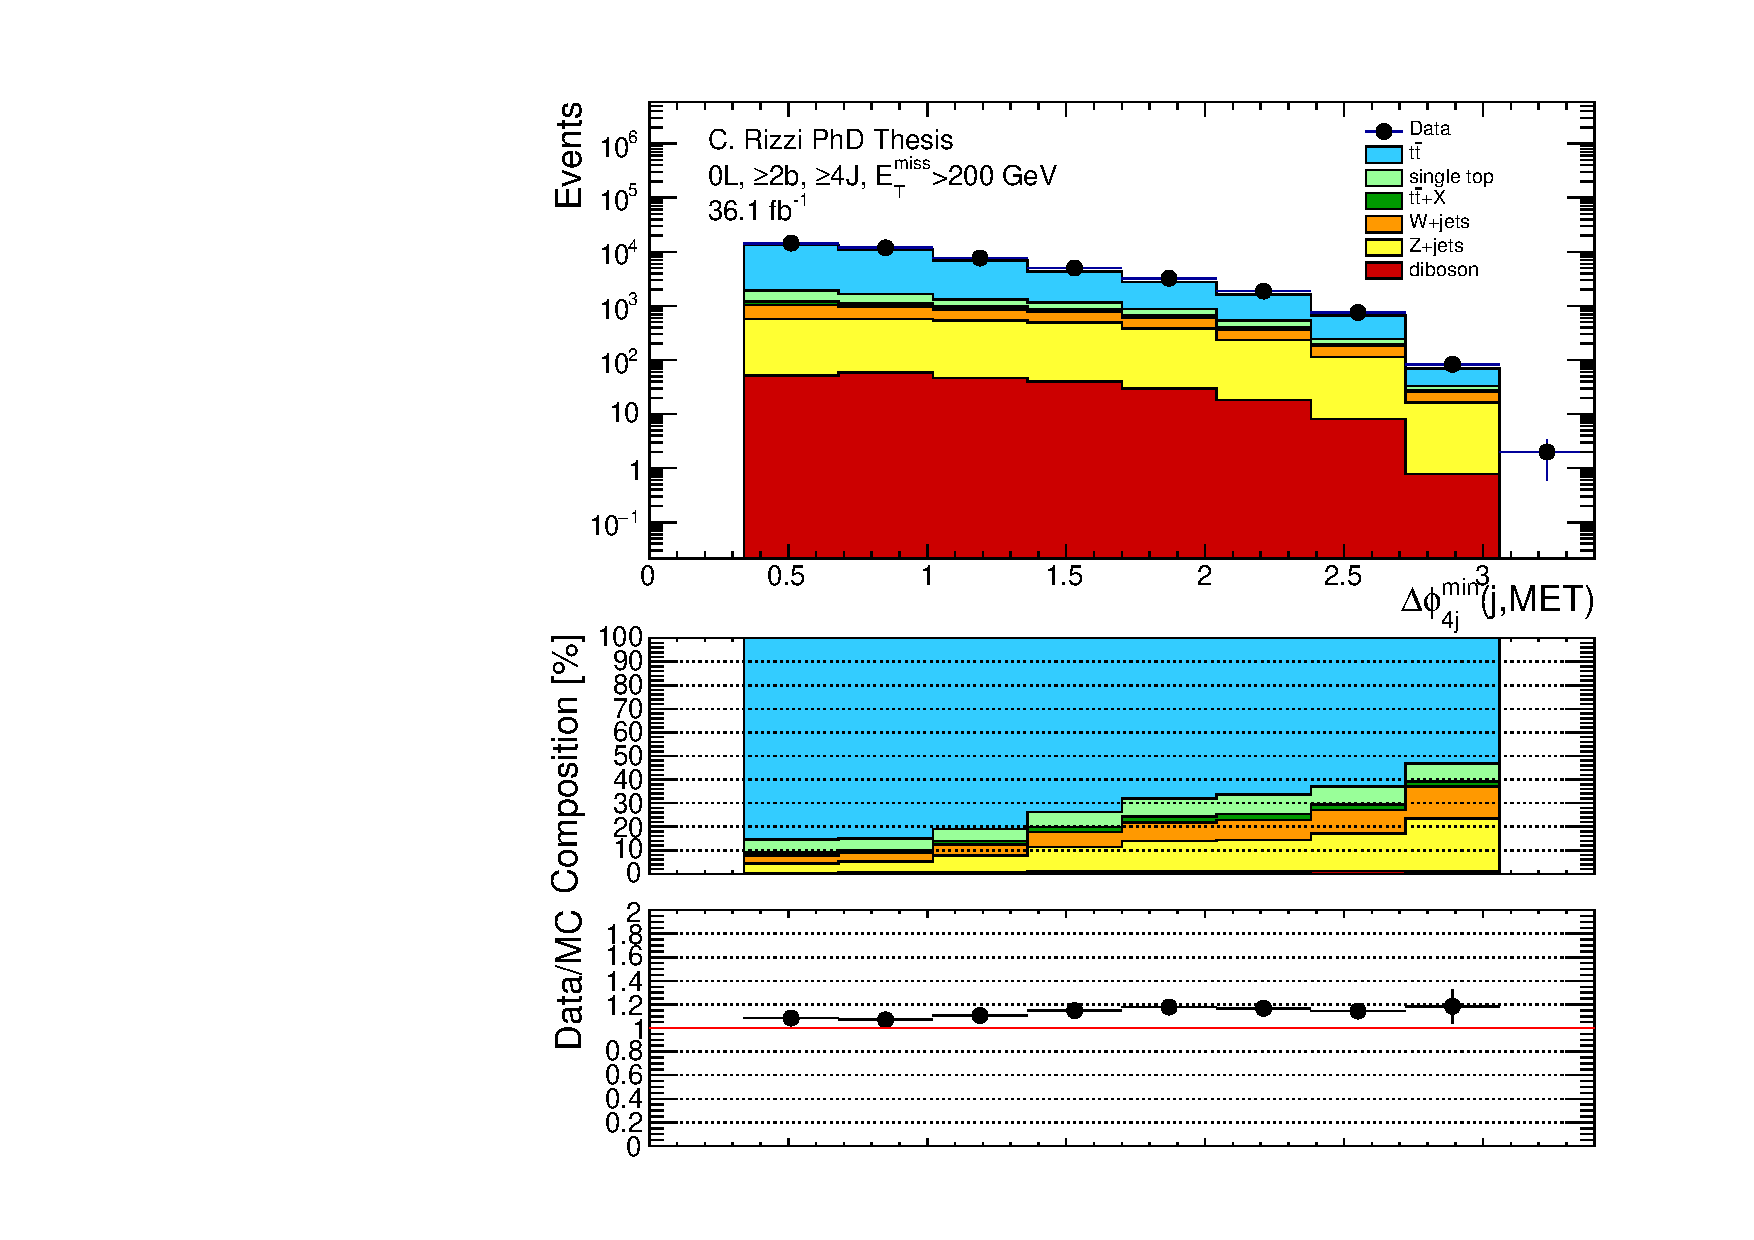
\includegraphics[width=0.45\textwidth]{figures/strong_prod/data_mc/0L_2bin/data_mc_dphi_min.pdf}
\label{fig:strong:datamc0L:mT}}
\subfigure[\mtb]{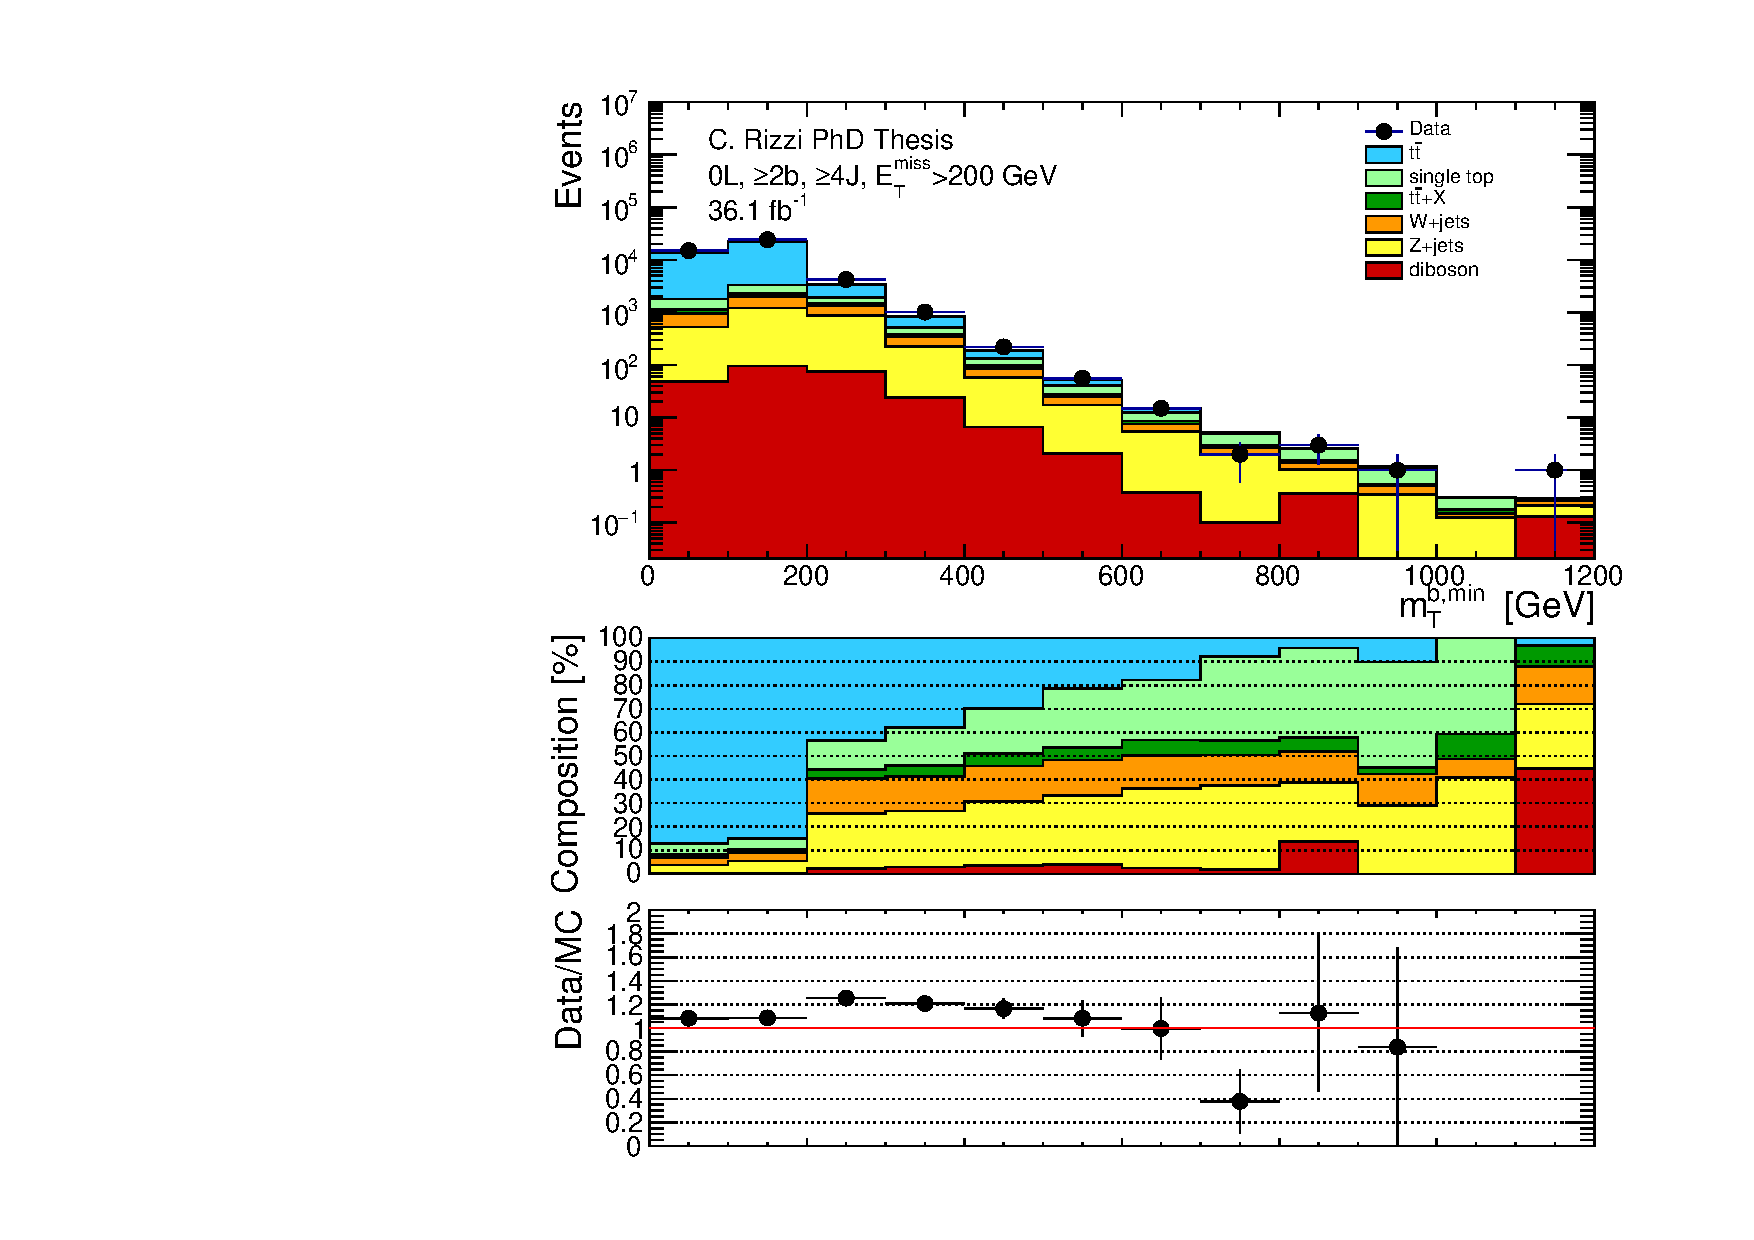
\includegraphics[width=0.45\textwidth]{figures/strong_prod/data_mc/0L_2bin/data_mc_mTb_min.pdf}
\label{fig:strong:datamc0L:mTb_min}}
\caption{Data-MC comparison in the 0-lepton preselection.
}
\label{fig:strong:datamc0L_a}
\end{figure*}

\begin{figure*}[htbp]
\centering 
\subfigure[\njet]{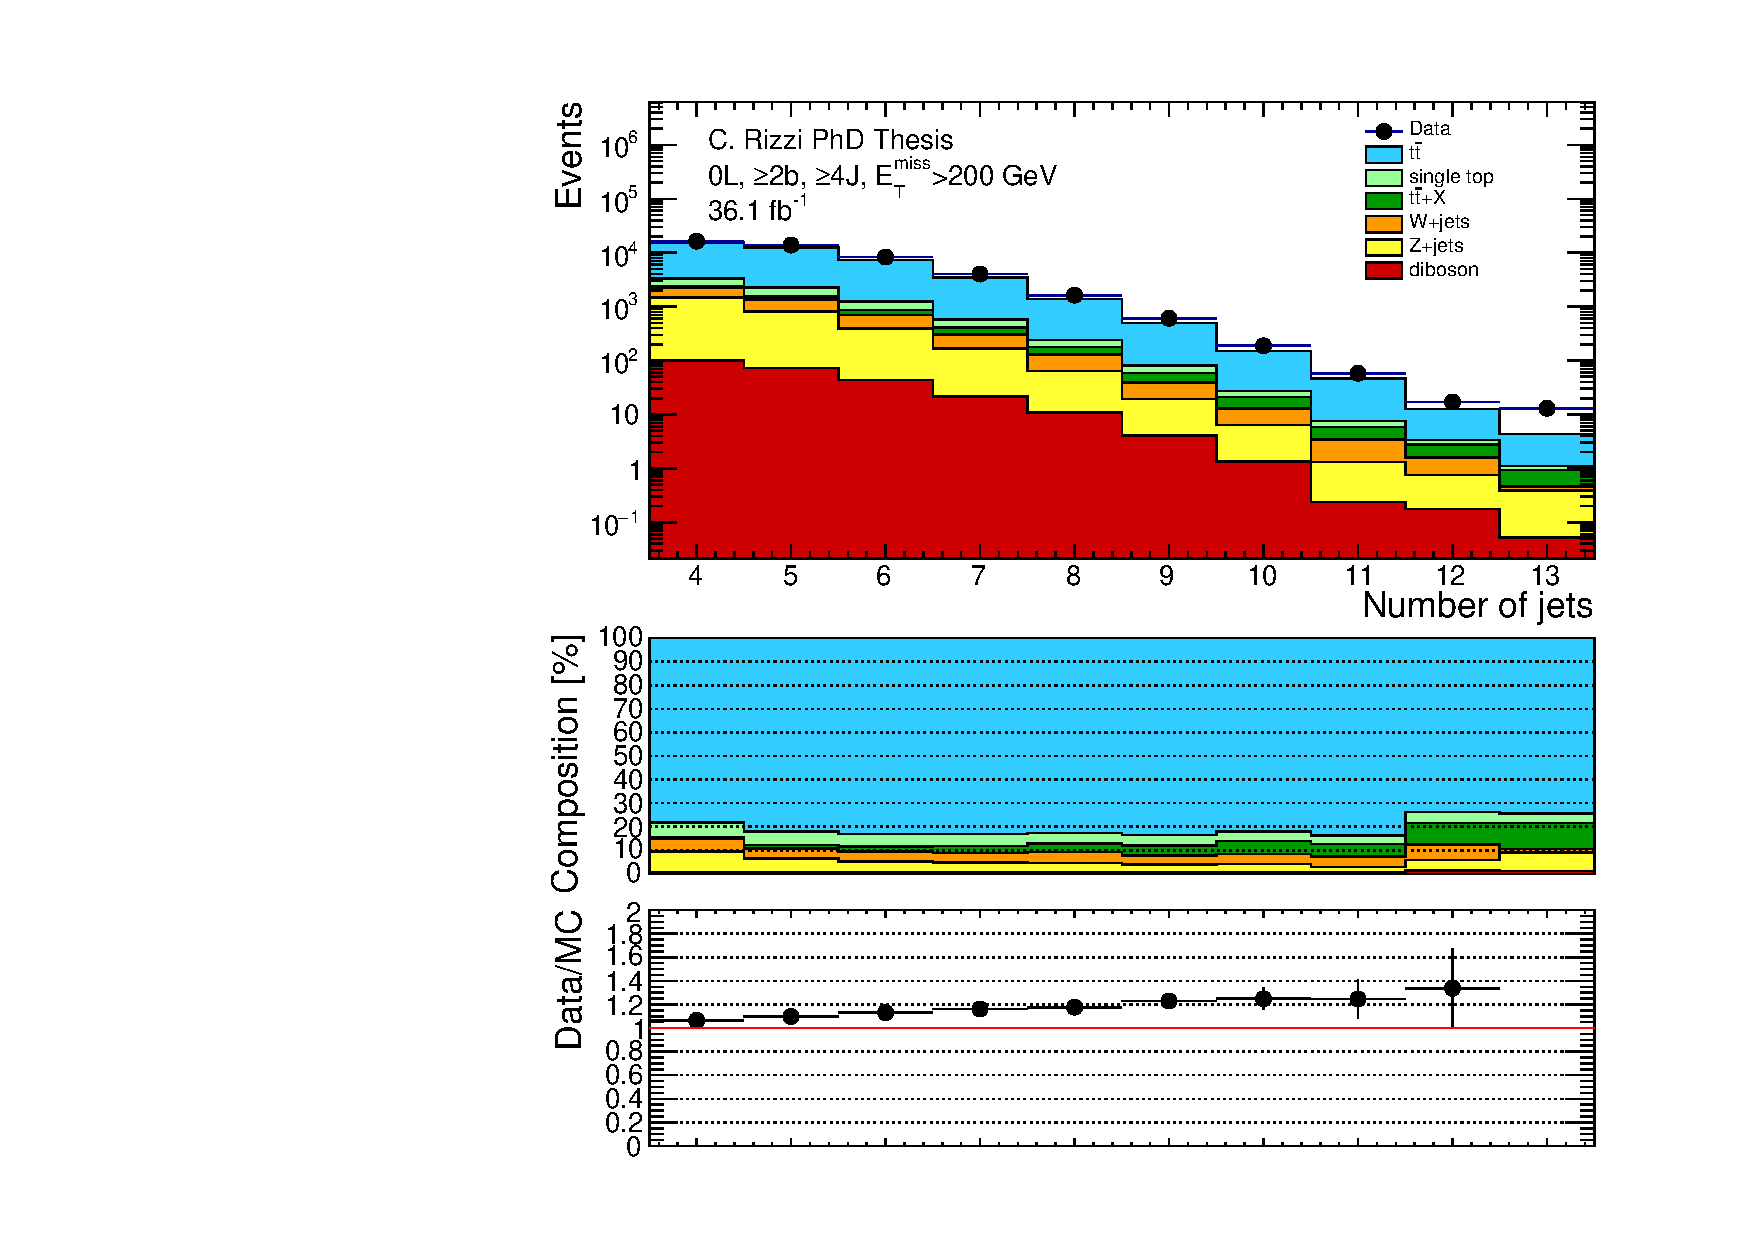
\includegraphics[width=0.45\textwidth]{figures/strong_prod/data_mc/0L_2bin/data_mc_jets_n.pdf}
\label{fig:strong:datamc0L:jets_n}}
\subfigure[\nbjet]{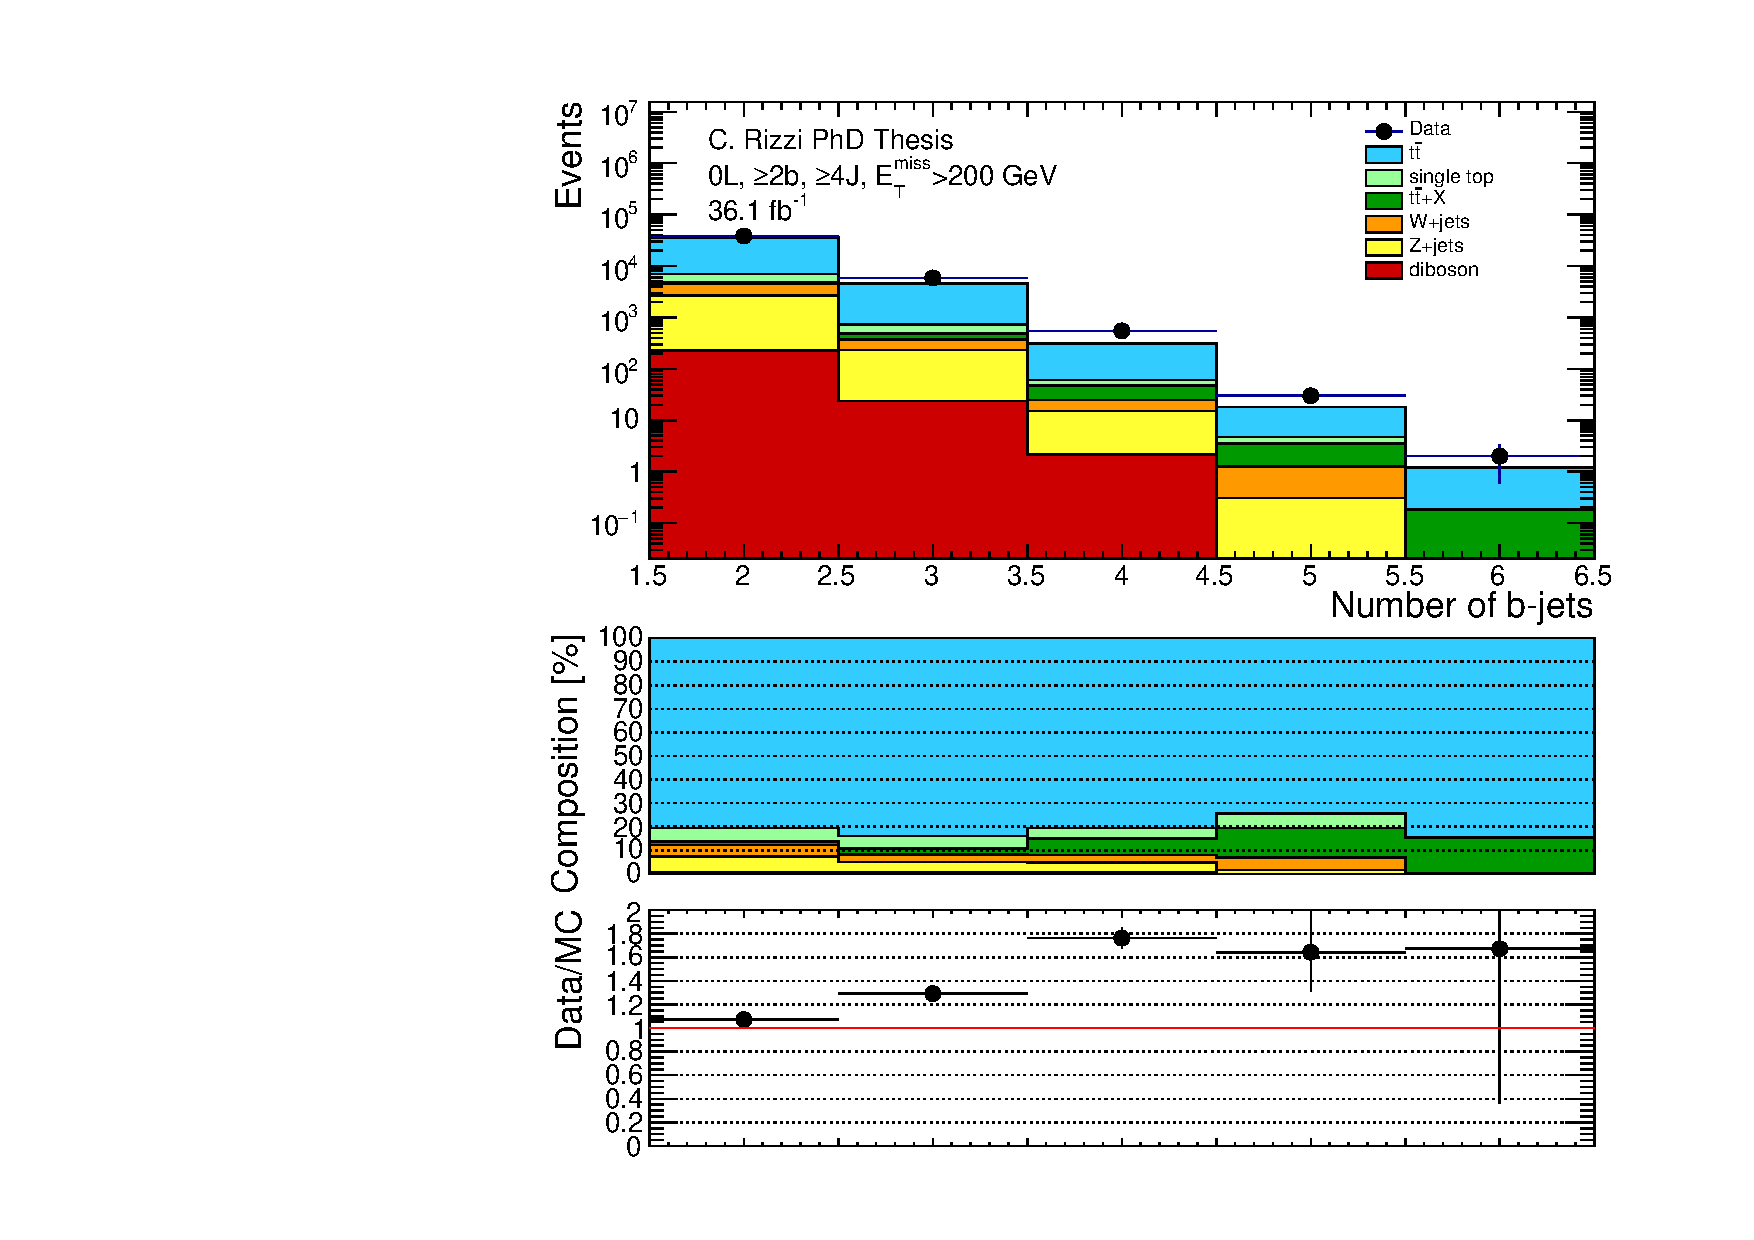
\includegraphics[width=0.45\textwidth]{figures/strong_prod/data_mc/0L_2bin/data_mc_bjets_n.pdf}
\label{fig:strong:datamc0L:bjets_n}}\\
\subfigure[\pt jet$_1$]{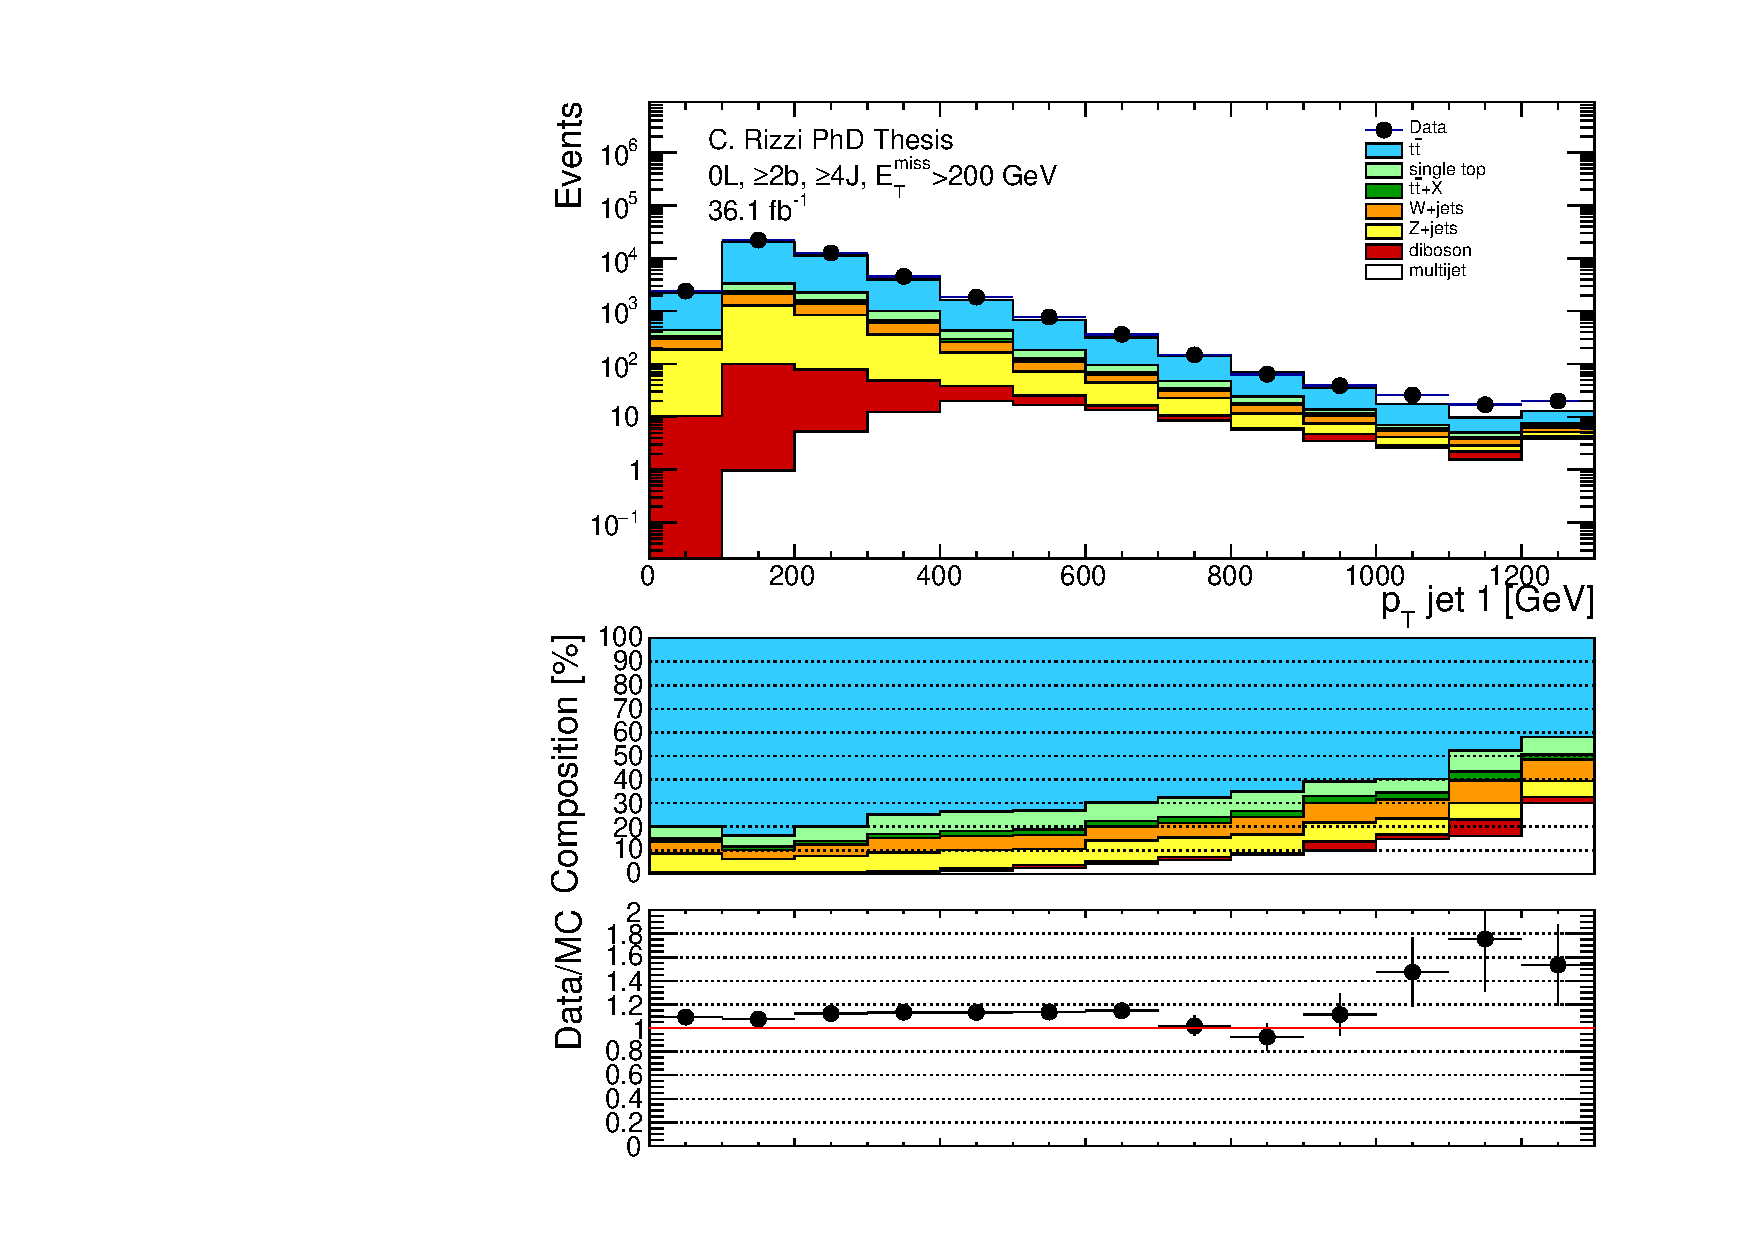
\includegraphics[width=0.45\textwidth]{figures/strong_prod/data_mc/0L_2bin/data_mc_pt_jet_1.pdf}
\label{fig:strong:datamc0L:pt_jet_1}}
\subfigure[\pt jet$_2$]{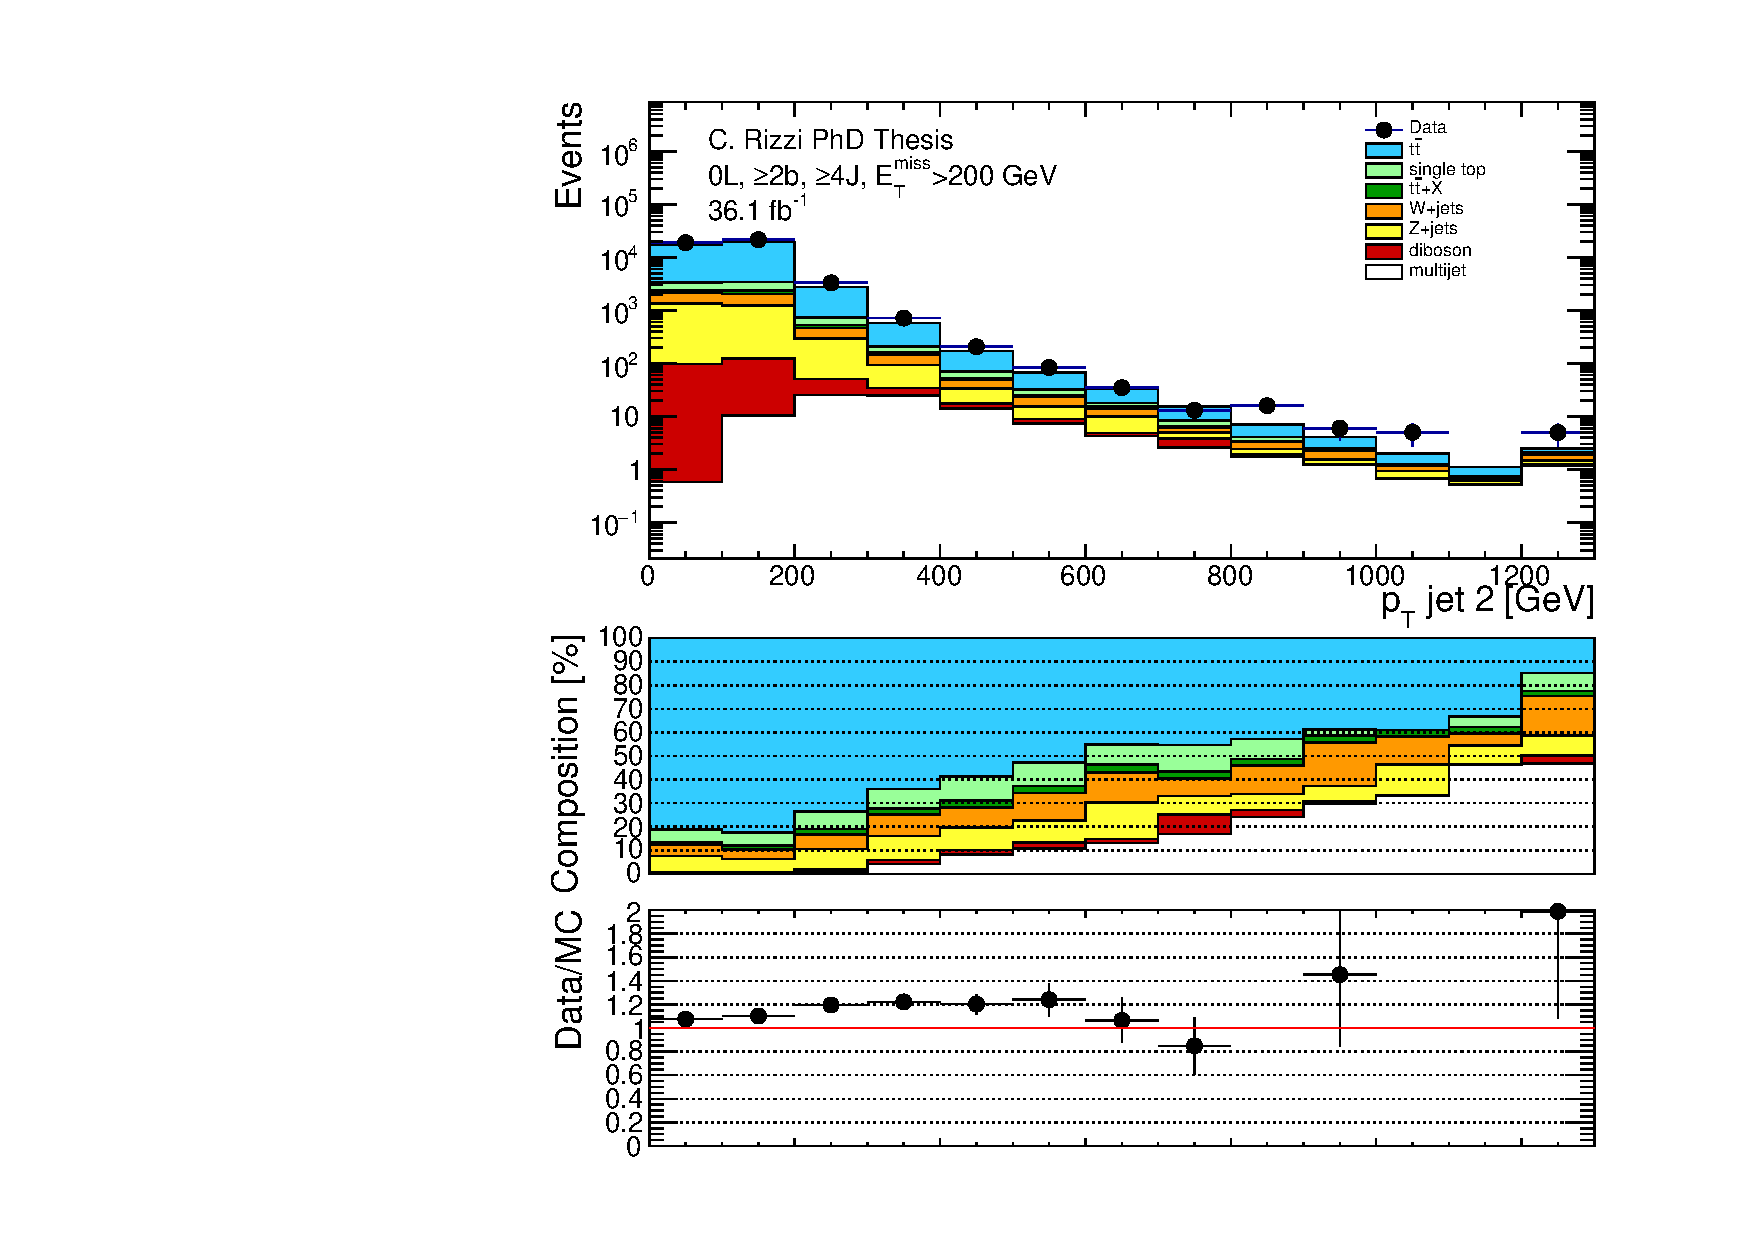
\includegraphics[width=0.45\textwidth]{figures/strong_prod/data_mc/0L_2bin/data_mc_pt_jet_2.pdf}
\label{fig:strong:datamc0L:pt_jet_2}}\\
\subfigure[\pt lep$_1$]{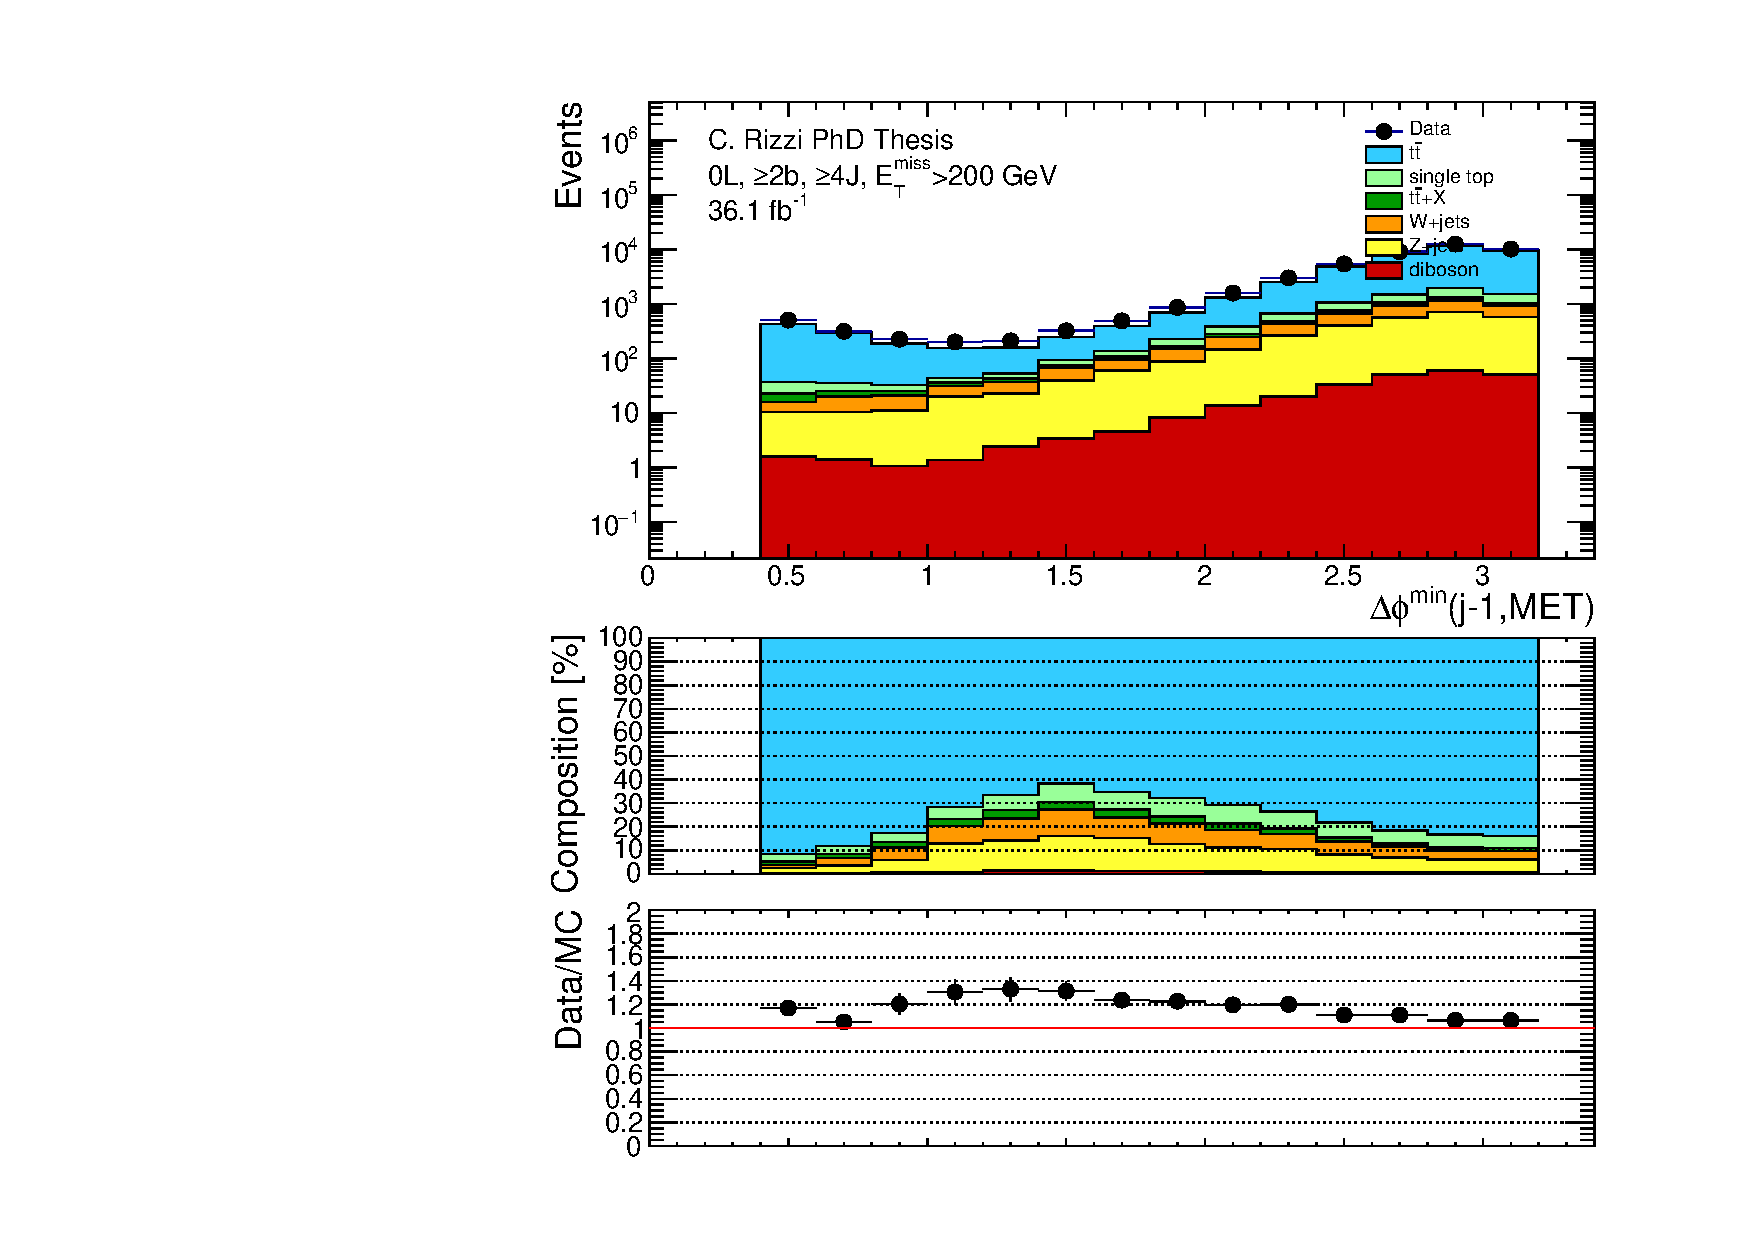
\includegraphics[width=0.45\textwidth]{figures/strong_prod/data_mc/0L_2bin/data_mc_dphi_1jet.pdf}
\label{fig:strong:datamc0L:ptlep1}}
\subfigure[\pt b-jet$_1$]{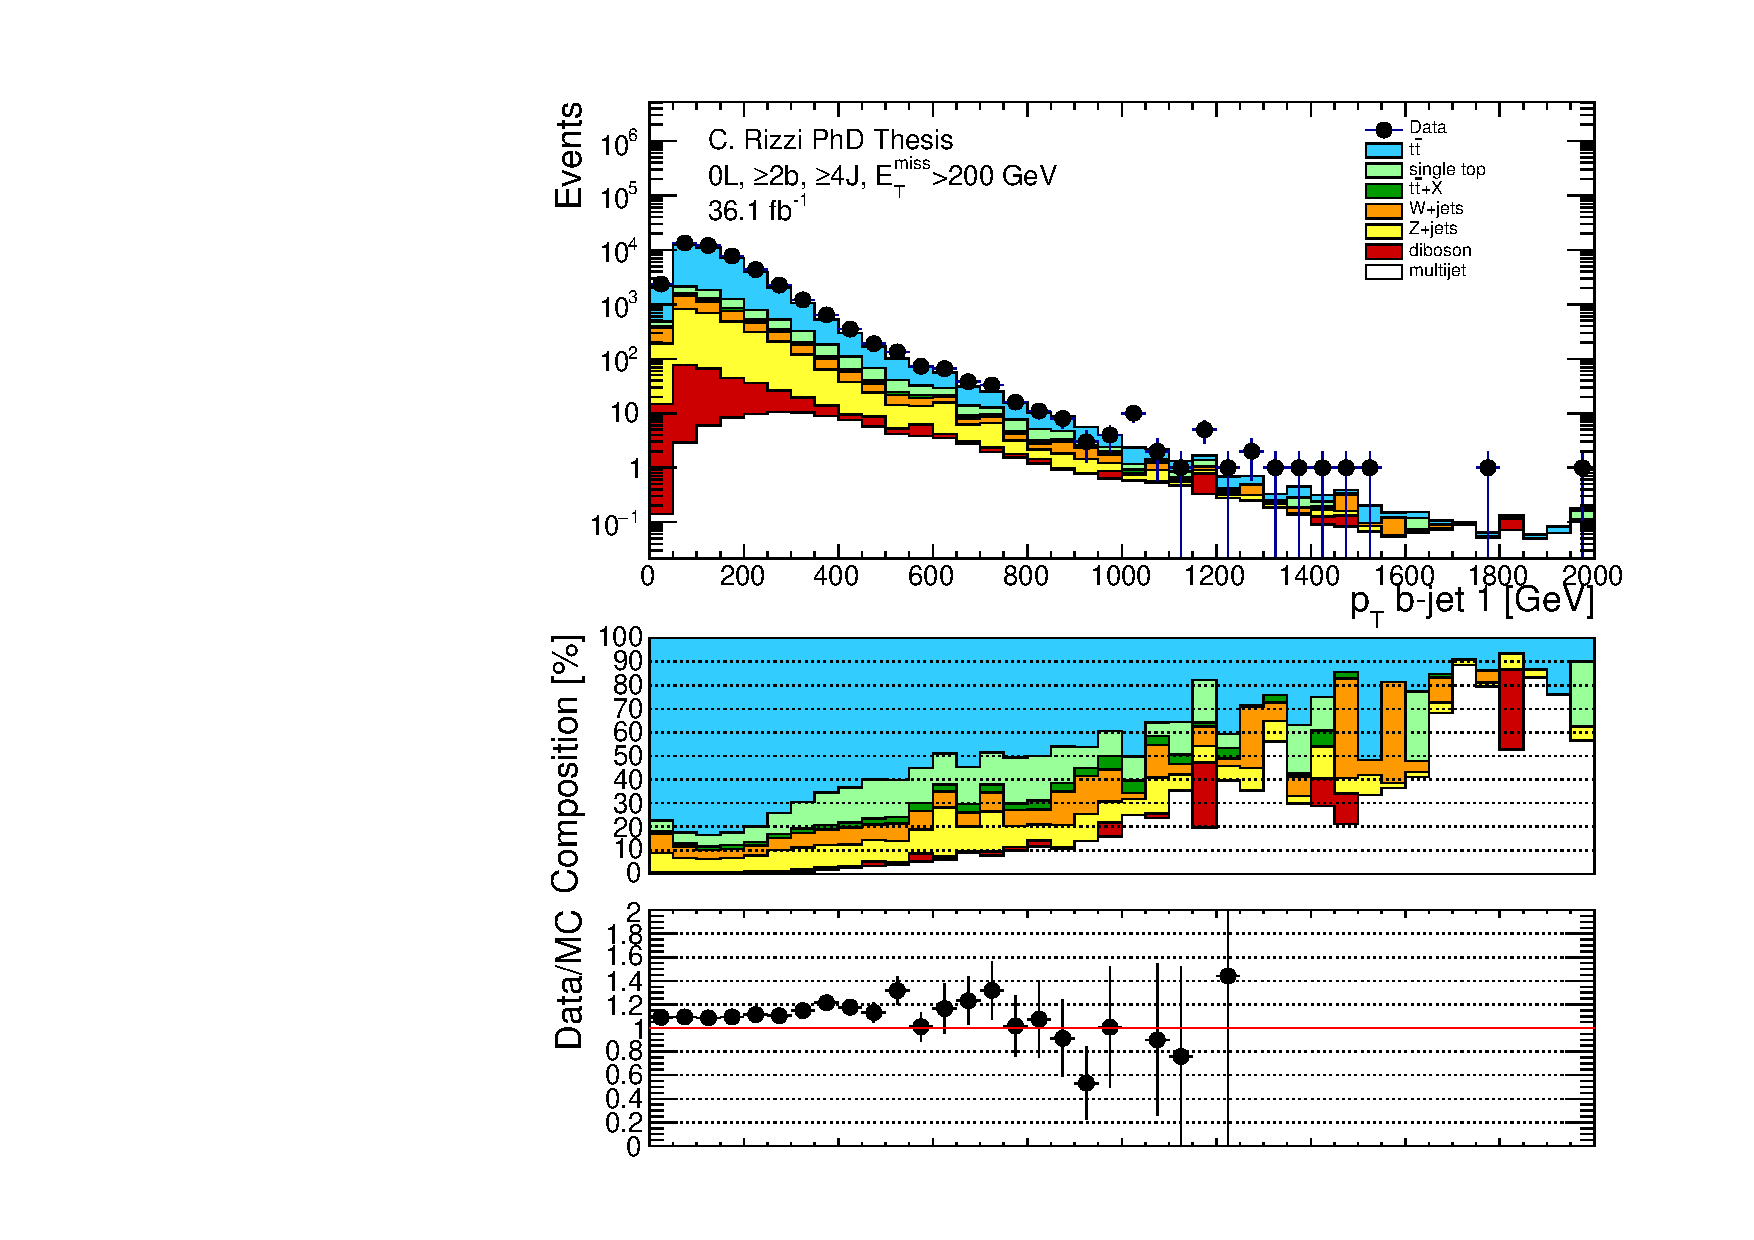
\includegraphics[width=0.45\textwidth]{figures/strong_prod/data_mc/0L_2bin/data_mc_pt_bjet_1.pdf}
\label{fig:strong:datamc0L:pt_bjet_1}}
\caption{Data-MC comparison in the 0-lepton preselection.
}
\label{fig:strong:datamc0L_b}
\end{figure*}
